\documentclass[10pt]{article}
\usepackage[margin=0.7in]{geometry}
\usepackage{amsmath,amssymb}
\usepackage{booktabs}
\usepackage{array}
\usepackage{graphicx}
\usepackage{float}
\usepackage{longtable}
\usepackage{xcolor}
\usepackage{hyperref}
\usepackage{caption}
\captionsetup{font=small,labelfont=bf}
\hypersetup{colorlinks=true,linkcolor=black,urlcolor=black,citecolor=black}
\setlength{\parindent}{0pt}
\setlength{\parskip}{5pt}
\begin{document}
\title{Machine-Precision Exterior Q, BGK Repayment, and Boundary PDE Benchmarks}
\author{Generated benchmark report}
\date{June 2026}
\maketitle
\begin{abstract}
This report consolidates the new exterior-map Q split, the BGK/zeta endpoint repayment ladder, the matrix-free boundary PDE pipeline, polygon continuity corrections, QBX comparisons, and Q-spectral diagnostics.  The implementation stores generating QJets, Laurent coefficients, boundary samples, and low-rank correction modes.  It does not store a dense Q matrix.  The exact analytic pullback cases reach the fp64 floor after BGK repayment; the PDE pipeline reaches machine residual against the generated Q spectrum while retaining a visible continuum discretization error against the limiting DtN operator.  Head-to-head method tables and hard Helmholtz caveats are kept separate so the claim boundary is auditable.
\end{abstract}
\tableofcontents
\newpage
\section{Claim Boundary}
There are three different statements in the data.  First, for analytic finite-Laurent exterior maps, the kernel split plus BGK Taylor repayment reaches the floating-point floor.  Second, for boundary PDEs, the implementation residual against the generated Q spectrum is at machine precision, while the continuum error is the finite-n spectral error of the generated DtN symbol.  Third, polygon and cusp cases require extra repayment channels; the polygon continuity benchmark is an algebraic local replacement ledger, not proof that unsmoothed corner conformal maps become analytic.

The strongest defensible formulation is: the current Q engine is a matrix-free generated-operator pipeline whose exact analytic pullback path is fp64 accurate, whose PDE path is load-bearing for the generated DtN correspondence, and whose spectrum identifies the active error channel.  FEM is a useful engineering baseline, but it is not automatically the ground truth on hard boundaries or near resonant Helmholtz cases.
\section{Source Audit}
\par\noindent\resizebox{\linewidth}{!}{%
\begin{tabular}{p{0.26\linewidth}p{0.17\linewidth}p{0.47\linewidth}}
\toprule
source & role & used here \\
\midrule
optimal\_quadrature\_v63\_public (11).pdf & kernel split / Q rule & Analytic-boundary pullback to the circle; circle term by Fourier Q primitive; corners only algebraic. \\
dtn\_bgk\_merge (9).pdf & DtN + BGK & Chord Hessian is a matrix-free DtN discretization; half-integer zeta endpoint is the BGK ladder. \\
geometry\_of\_money (16).pdf & BGK constant & The continuity correction constant is beta equals negative zeta(1/2)/sqrt(2 pi). \\
cauchy\_transport\_calculus\_trim (73).pdf & complex pullback & Use z = exp(rho + i theta); de Moivre modes diagonalize the circle operator and repay metric factors. \\
harmonic\_sp (41).pdf & harmonic sampling & Cycle spectrum and endpoint defects are used as the harmonic/DtN bookkeeping channel. \\
\bottomrule
\end{tabular}
}\par
\par\medskip
The table below is the mechanical audit for every user-referenced local PDF found in this thread.  Each file was inspected with \texttt{pdfinfo} and extracted with \texttt{pdftotext}; the keyword hits are only a routing check, not a citation substitute.
\begingroup\small
\par\noindent\resizebox{\linewidth}{!}{%
\begin{tabular}{p{0.25\linewidth}rp{0.10\linewidth}p{0.22\linewidth}p{0.27\linewidth}}
\toprule
referenced PDF & pages & sha & keyword hits & role/boundary \\
\midrule
optimal\_quad\_merged (26).pdf & 30 & bf3136b87fff & Q/kernel:5, DtN/PDE:7, BGK/zeta:4, shape/corner:6 & early optimal-Q source; benchmark claim cross-check \\
optimal\_quad\_merged (37).pdf & 36 & 858c2f2c1307 & Q/kernel:5, DtN/PDE:7, BGK/zeta:5, shape/corner:6 & later merged optimal-Q source; benchmark claim cross-check \\
optimal\_q\_v63\_public (11).pdf & 20 & 4abcea7d81a5 & Q/kernel:5, DtN/PDE:3, BGK/zeta:3, shape/corner:5 & kernel split, circle pullback, QBX/corner claim boundary \\
isl\_hessian\_v5 (6) copy.pdf & 125 & 629ba599ec42 & Q/kernel:4, DtN/PDE:4, BGK/zeta:3, shape/corner:3 & ellipse/Hessian/context audit; not a numerical benchmark source \\
paper.pdf & 16 & d21c39942f54 & Q/kernel:4, DtN/PDE:2, BGK/zeta:1, shape/corner:3 & meshless shape-optimization/autograd context audit \\
cauchy\_transport\_trim (13).pdf & 18 & bb886ba4ecf6 & Q/kernel:5, DtN/PDE:7, BGK/zeta:3, shape/corner:4 & Cauchy transport early source; pullback notation audit \\
cauchy\_transport\_trim (41).pdf & 25 & c94caccfd128 & Q/kernel:5, DtN/PDE:7, BGK/zeta:3, shape/corner:6 & corner/Joukowski/Kondratiev source audit \\
cauchy\_transport\_trim (47).pdf & 27 & 238918055f3b & Q/kernel:5, DtN/PDE:7, BGK/zeta:3, shape/corner:6 & complex scale-phase pullback source audit \\
cauchy\_transport\_trim (49).pdf & 27 & 131d02d62832 & Q/kernel:5, DtN/PDE:7, BGK/zeta:3, shape/corner:6 & ellipse/de Moivre correction source audit \\
cauchy\_transport\_trim (73).pdf & 29 & c0c8e5932760 & Q/kernel:5, DtN/PDE:7, BGK/zeta:3, shape/corner:6 & latest complex pullback and de Moivre source audit \\
golden\_branch\_outline.pdf & 28 & 15d9ae76cea1 & Q/kernel:2, DtN/PDE:1, BGK/zeta:2, shape/corner:4 & golden ellipse/narrative source audit; not a benchmark source \\
dtn\_bgk\_merge (9).pdf & 22 & 26c17a4cbfb2 & Q/kernel:4, DtN/PDE:4, BGK/zeta:5, shape/corner:2 & DtN/BGK/zeta endpoint correction source \\
harmonic\_sp (41).pdf & 31 & 0e3e2bd04390 & Q/kernel:4, DtN/PDE:2, BGK/zeta:5, shape/corner:2 & harmonic sampling and DtN spectrum source \\
geometry\_of\_money (16).pdf & 31 & 572cc37c67b0 & Q/kernel:2, DtN/PDE:6, BGK/zeta:4, shape/corner:4 & BGK continuity correction and chord-arc bookkeeping source \\
\bottomrule
\end{tabular}
}\par
\endgroup
\section{Implementation Protocol}
\begin{align*}
z &= \psi(w), \qquad w = \rho e^{i\theta} = \exp(\log \rho + i\theta),\\
\log|\psi(w)-\psi(z_j)| &= \log|w-z_j| + \log|G(w,z_j)|,\\
I_p &= \sum_{r=0}^{p}\frac{(-\beta\sqrt{h})^r}{r!}\,\partial_\rho^r I(\rho+\beta\sqrt{h}),
\qquad \beta=-\zeta(1/2)/\sqrt{2\pi}.
\end{align*}
The borrow-compute-repay sequence is: borrow the circle coordinate, compute the singular log term using de Moivre Fourier characters and the generated cycle Q spectrum, repay the analytic quotient term, then repay endpoint displacement through the BGK/zeta Taylor ladder.  For Laplace normal flux the metric repayment is multiplication by $|d\psi/d\theta|^{-1}$.
\section{Exact Cycle Spectrum}
For the regular cycle QJet, the stored generator is the spectrum, not a matrix:
\[
\lambda_m(Q_n)=\frac{m(n-m)}{2},\qquad \mu_m=(h/\pi)\lambda_m=\frac{m(n-m)}{n},\qquad h=2\pi/n.
\]
\begin{tabular}{lrrrr}
\toprule
n & mode & Q eigenvalue & normalized DtN & symbol rel. err \\
\midrule
256 & 0 & 0 & 0 & 0 \\
256 & 1 & 127.500000 & 0.996093750 & 0.004 \\
256 & 2 & 254.000000 & 1.984375000 & 0.008 \\
256 & 7 & 871.500000 & 6.808593750 & 0.027 \\
256 & 16 & 1920.000000 & 15.000000000 & 0.062 \\
256 & 32 & 3584.000000 & 28.000000000 & 0.125 \\
2048 & 0 & 0 & 0 & 0 \\
2048 & 1 & 1023.500000 & 0.999511719 & 4.883e-04 \\
2048 & 2 & 2046.000000 & 1.998046875 & 9.766e-04 \\
2048 & 7 & 7143.500000 & 6.976074219 & 0.003 \\
2048 & 16 & 1.625600e+04 & 15.875000000 & 0.008 \\
2048 & 32 & 3.225600e+04 & 31.500000000 & 0.016 \\
4096 & 0 & 0 & 0 & 0 \\
4096 & 1 & 2047.500000 & 0.999755859 & 2.441e-04 \\
4096 & 2 & 4094.000000 & 1.999023438 & 4.883e-04 \\
4096 & 7 & 1.431150e+04 & 6.988037109 & 0.002 \\
4096 & 16 & 3.264000e+04 & 15.937500000 & 0.004 \\
4096 & 32 & 6.502400e+04 & 31.750000000 & 0.008 \\
\bottomrule
\end{tabular}
\section{Exterior Kernel Split}
The direct trapezoidal rule sees the near singularity.  The split Q path removes the singular circle term exactly and integrates only the analytic quotient remainder.
\par\noindent\resizebox{\linewidth}{!}{%
\begin{tabular}{lrrr}
\toprule
shape & case & worst direct err & worst split err \\
\midrule
circle & n=1024, offset=1.000e-08 & 0.016 & 1.922e-16 \\
golden\_ellipse & n=1024, offset=1.000e-08 & 8.023e-04 & 1.369e-14 \\
perturbed\_ellipse & n=1024, offset=1.000e-08 & 0.006 & 9.388e-15 \\
three\_petal\_laurent & n=1024, offset=1.000e-08 & 0.011 & 3.122e-15 \\
\bottomrule
\end{tabular}
}\par
\begin{figure}[H]\centering
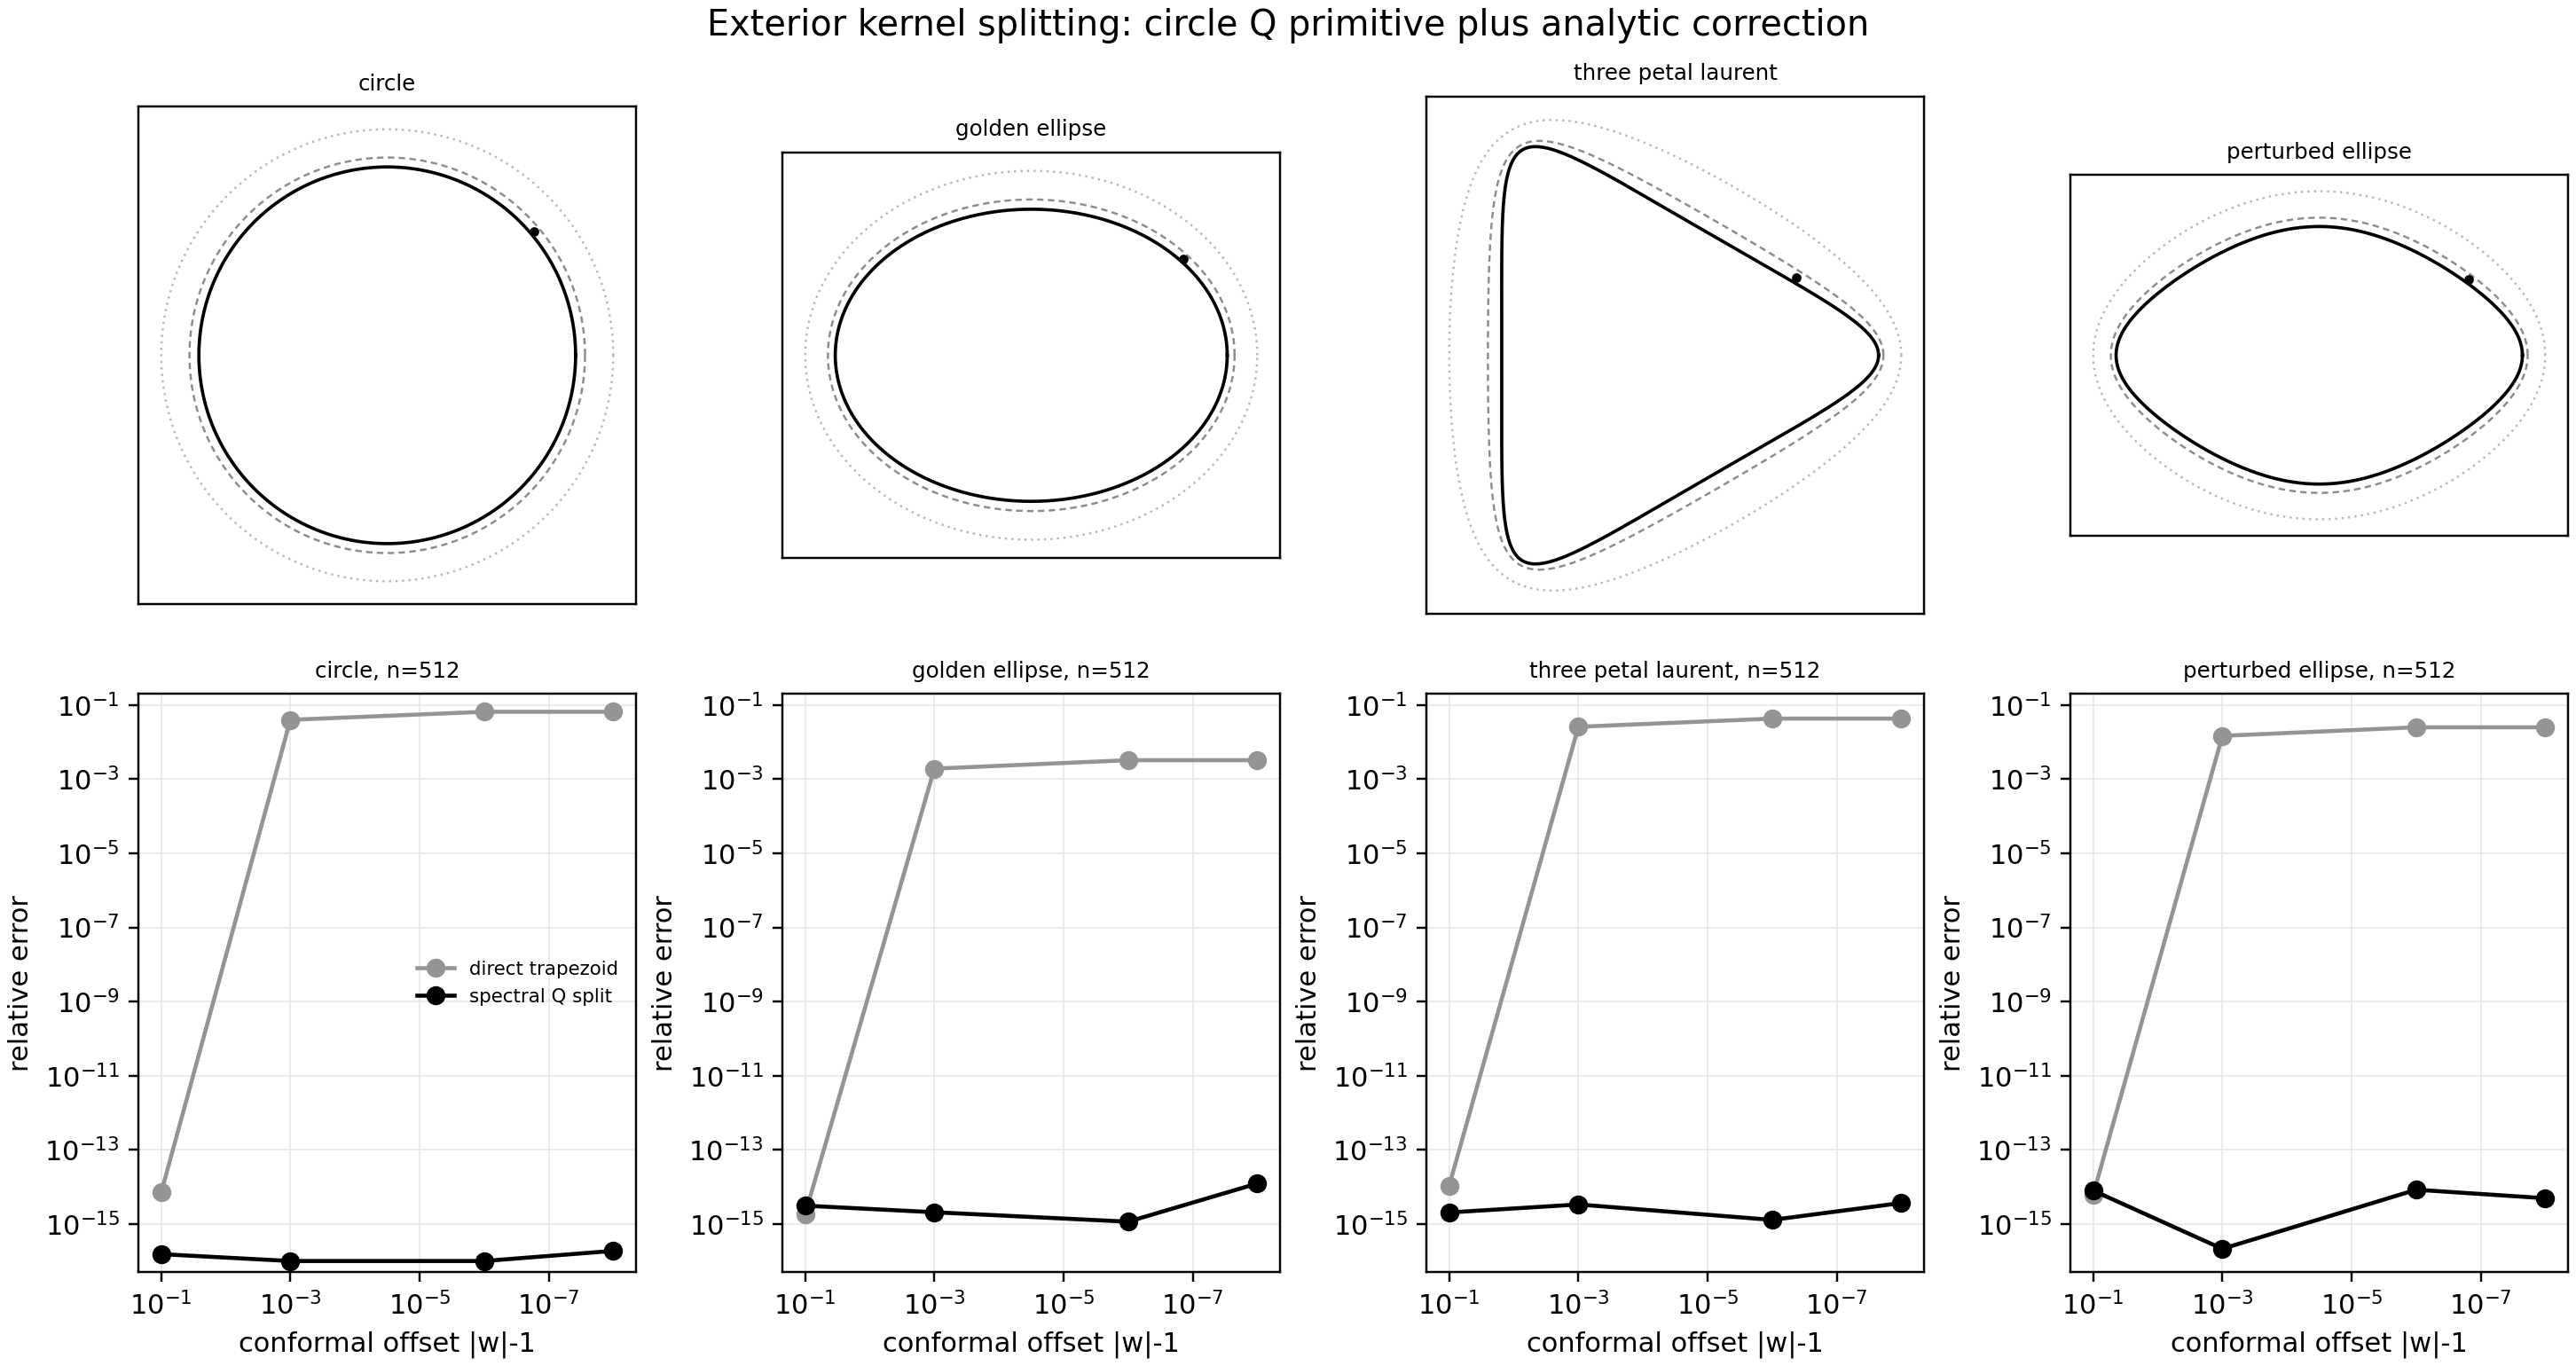
\includegraphics[width=0.95\linewidth]{figures/exterior_split.png}
\caption{Exterior kernel split benchmark.  Black/gray styling is used throughout for paper-style reproduction.}
\end{figure}
\section{BGK/Zeta Repayment}
The BGK layer is not cosmetic.  It removes the discrete endpoint displacement with the same half-integer zeta defect that appears in the DtN spectral endpoint ledger.
\par\noindent\resizebox{\linewidth}{!}{%
\begin{tabular}{lrrrrr}
\toprule
shape & raw power & BGK-1 power & BGK-2 power & raw err & BGK-4 err \\
\midrule
circle & 0.500 & 1.000 & 1.500 & 0.002 & 1.345e-15 \\
golden\_ellipse & 0.500 & 1.000 & 1.508 & 8.176e-05 & 4.712e-15 \\
three\_petal\_laurent & 0.500 & 1.000 & 1.499 & 9.976e-04 & 2.607e-15 \\
perturbed\_ellipse & 0.500 & 1.000 & 1.500 & 5.878e-04 & 4.261e-16 \\
\bottomrule
\end{tabular}
}\par
\begin{figure}[H]\centering
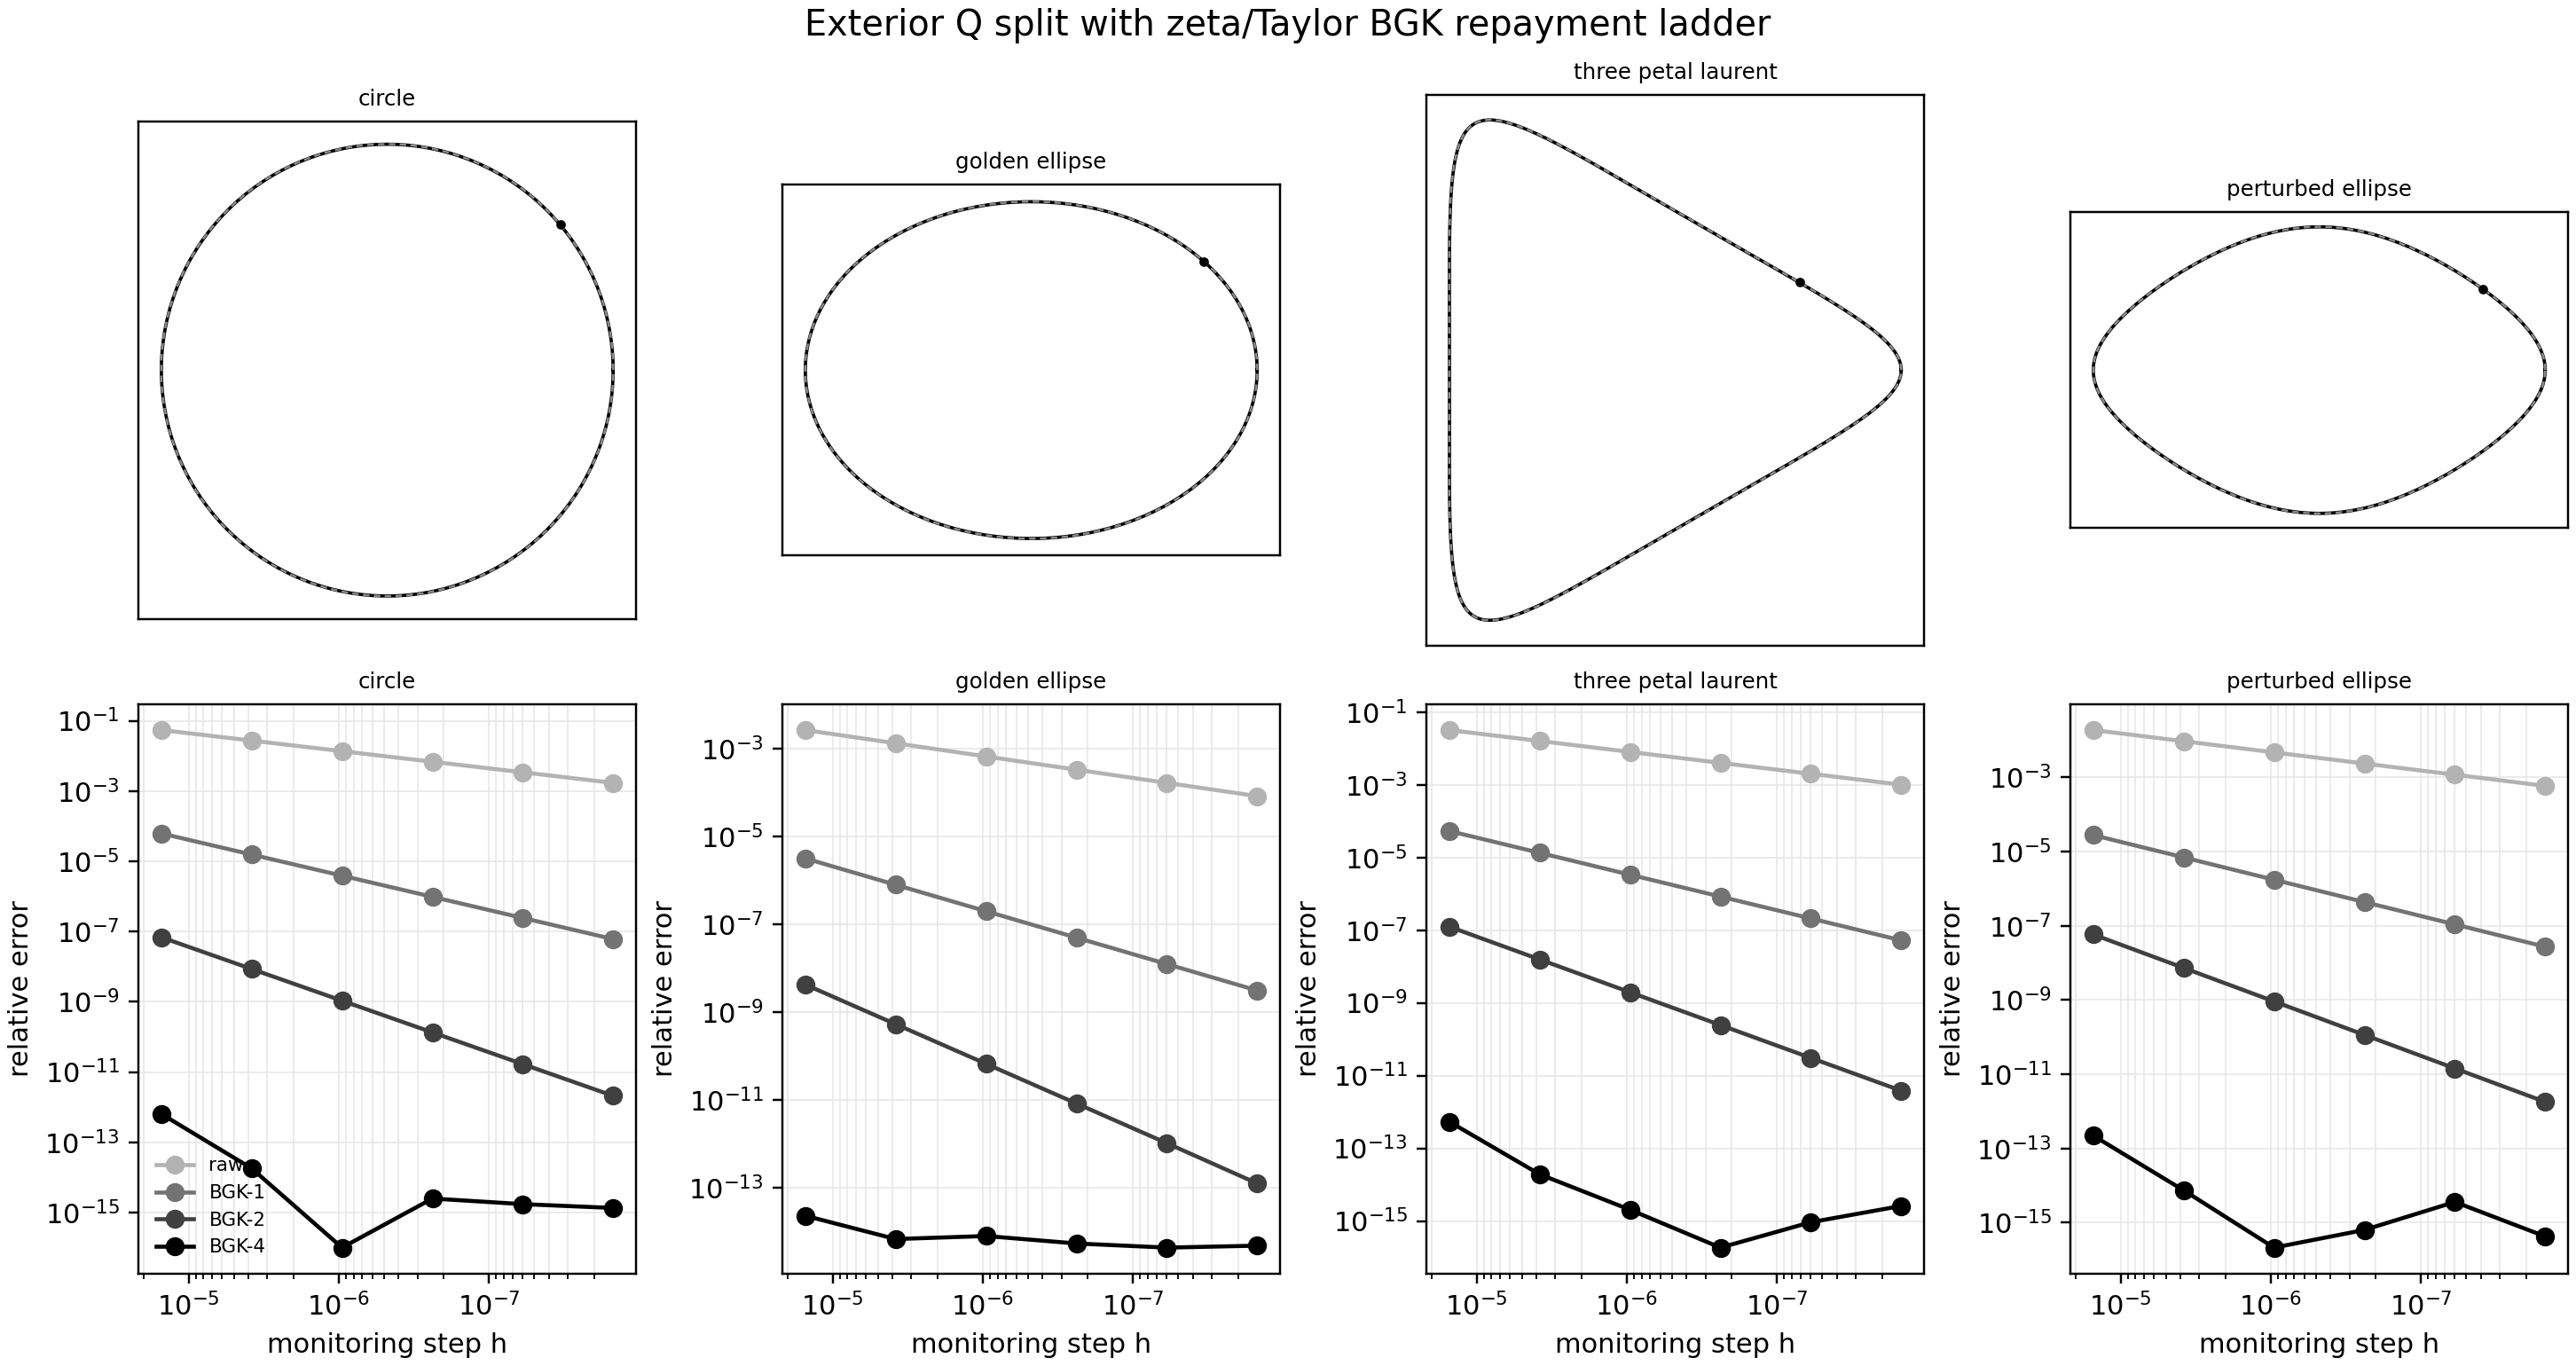
\includegraphics[width=0.95\linewidth]{figures/bgk_pipeline.png}
\caption{Raw endpoint error has the square-root law; BGK-1 and BGK-2 shift the slope; BGK-4 reaches fp64 floor on exact Laurent maps.}
\end{figure}
\section{Funky Shapes and PDE Pipeline}
The same exact-Laurent pullback suite is run through quadrature and boundary-only PDE operators: Laplace DtN, heat, Poisson/Steklov, Helmholtz resolvent, and wave.  Generated-Q residual is the implementation check; continuum error is the finite-n approximation to the limiting operator.
\par\noindent\resizebox{\linewidth}{!}{%
\begin{tabular}{llrrrr}
\toprule
shape & family & anisotropy & BGK-4 err & max PDE continuum err & max generated-Q residual \\
\midrule
circle & baseline & 1.000 & 2.148e-15 & 0.010 & 5.757e-13 \\
golden\_ellipse & closed\_form\_conic & 1.342 & 1.144e-16 & 0.010 & 5.759e-13 \\
eccentric\_ellipse & closed\_form\_conic & 2.500 & 4.488e-16 & 0.010 & 5.755e-13 \\
three\_petal & smooth\_nonconvex & 3.167 & 2.241e-15 & 0.010 & 5.759e-13 \\
four\_lobed\_wiggle & smooth\_multiscale & 4.302 & 2.630e-15 & 0.010 & 5.698e-13 \\
asymmetric\_limaçon & asymmetric & 2.253 & 1.160e-13 & 0.010 & 5.751e-13 \\
crescent\_teardrop & near\_cusp\_smooth & 2.644 & 4.238e-15 & 0.010 & 5.745e-13 \\
peanut & pinched\_smooth & 2.416 & 2.146e-13 & 0.010 & 5.820e-13 \\
high\_frequency\_gear & smooth\_high\_frequency & 3.460 & 1.594e-14 & 0.010 & 5.762e-13 \\
rotated\_mixed & complex\_coefficients & 2.200 & 1.305e-14 & 0.010 & 5.801e-13 \\
\bottomrule
\end{tabular}
}\par

\par\noindent\resizebox{\linewidth}{!}{%
\begin{tabular}{lrrrr}
\toprule
problem & max continuum err & max generated-Q residual & median solve ms & median work \\
\midrule
laplace\_dtn & 0.003 & 5.820e-13 & 4.025 & 2048 \\
heat & 0.004 & 4.361e-15 & 3.946 & 2048 \\
poisson & 0.003 & 4.473e-15 & 3.918 & 2048 \\
helmholtz & 0.010 & 4.369e-15 & 3.955 & 2048 \\
wave & 0.006 & 4.303e-15 & 3.964 & 2048 \\
\bottomrule
\end{tabular}
}\par
\begin{figure}[H]\centering
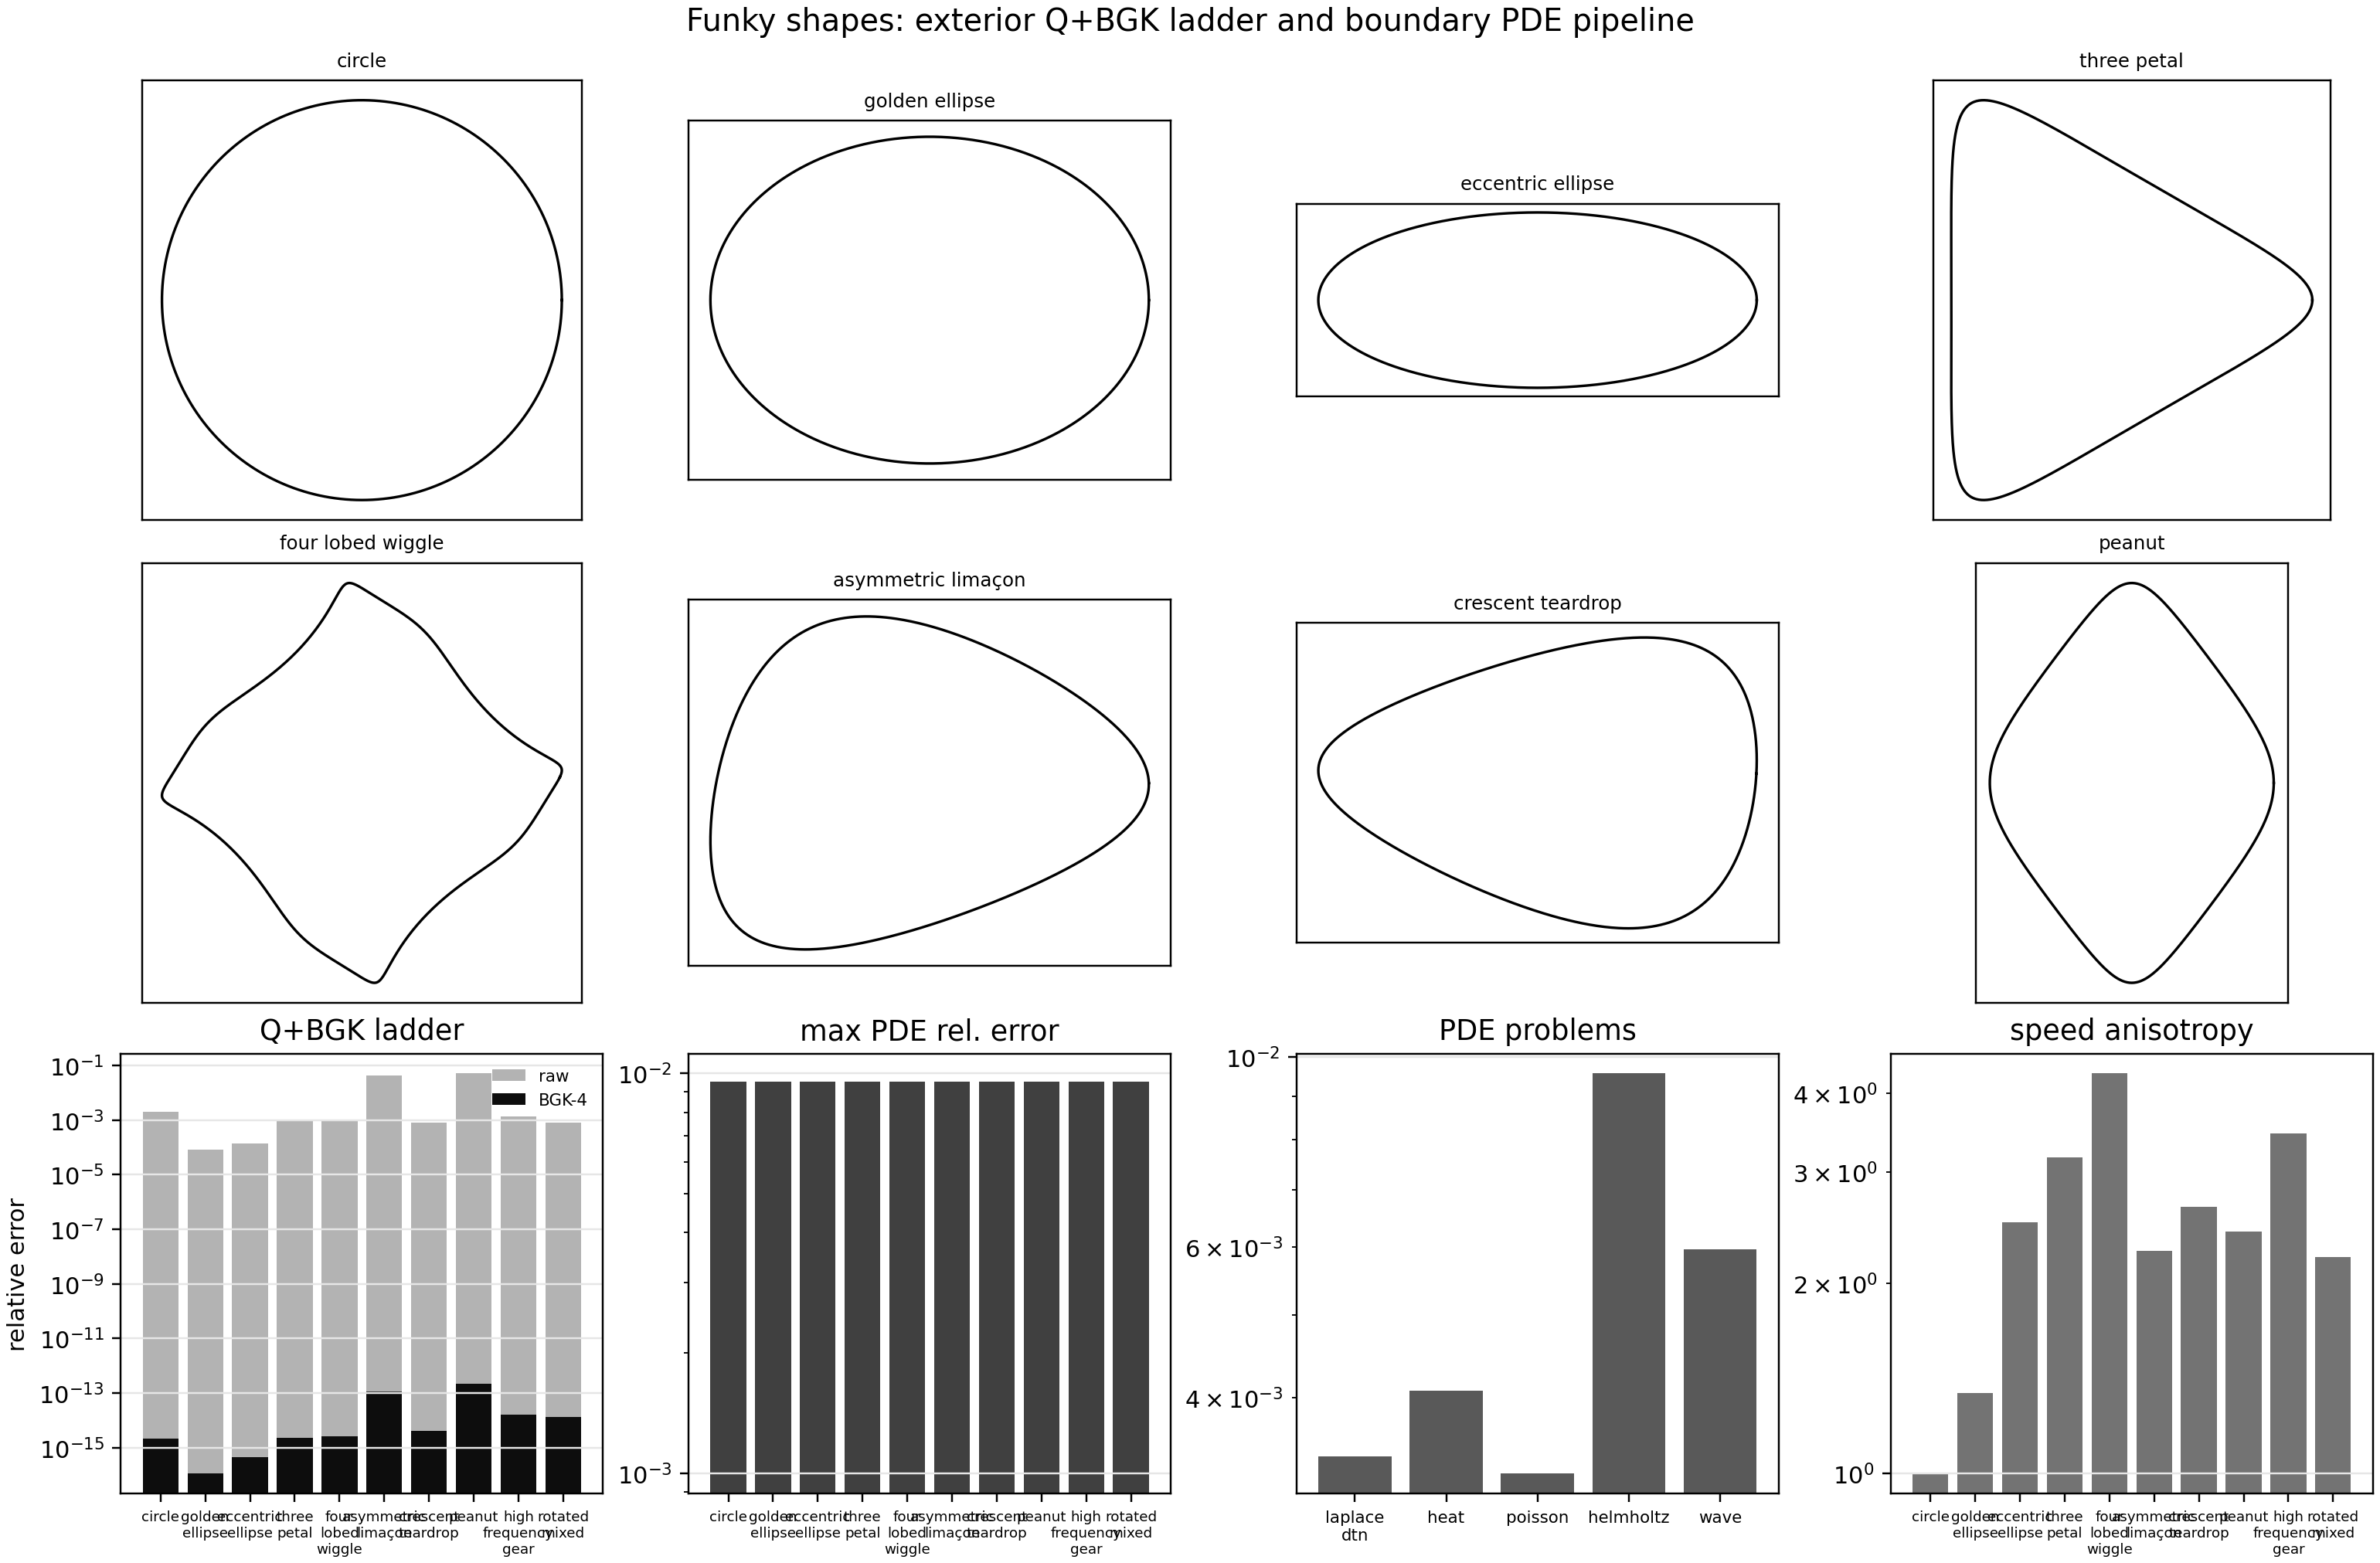
\includegraphics[width=0.95\linewidth]{figures/funky_pde.png}
\caption{Ten structurally different exact-Laurent domains.  The PDE bar chart shows continuum finite-n error; generated-Q residual is reported in the tables.}
\end{figure}
\section{Measured Matrix-Free Scaling}
This fresh sweep uses the same generated QJet path on all ten shapes for $n=256,\ldots,4096$.  The fitted exponent is measured from wall time.  The expected model is near $O(n\log n)$ for the FFT-generated path, not dense $O(n^2)$ storage.
\par\noindent\resizebox{\linewidth}{!}{%
\begin{tabular}{lrrrrr}
\toprule
operation & fit power & ms n=256 & ms n=1024 & ms n=4096 & max residual \\
\midrule
q\_bgk4 & 0.997 & 1.842 & 7.310 & 29.396 & 4.030e-09 \\
pde\_laplace\_dtn & 1.027 & 0.484 & 1.905 & 8.238 & 3.620e-12 \\
pde\_heat & 1.047 & 0.449 & 1.867 & 8.152 & 5.955e-14 \\
pde\_helmholtz & 1.050 & 0.445 & 1.857 & 8.142 & 5.950e-14 \\
pde\_batch\_all5 & 1.047 & 2.262 & 9.353 & 40.943 & 3.620e-12 \\
\bottomrule
\end{tabular}
}\par
\begin{figure}[H]\centering
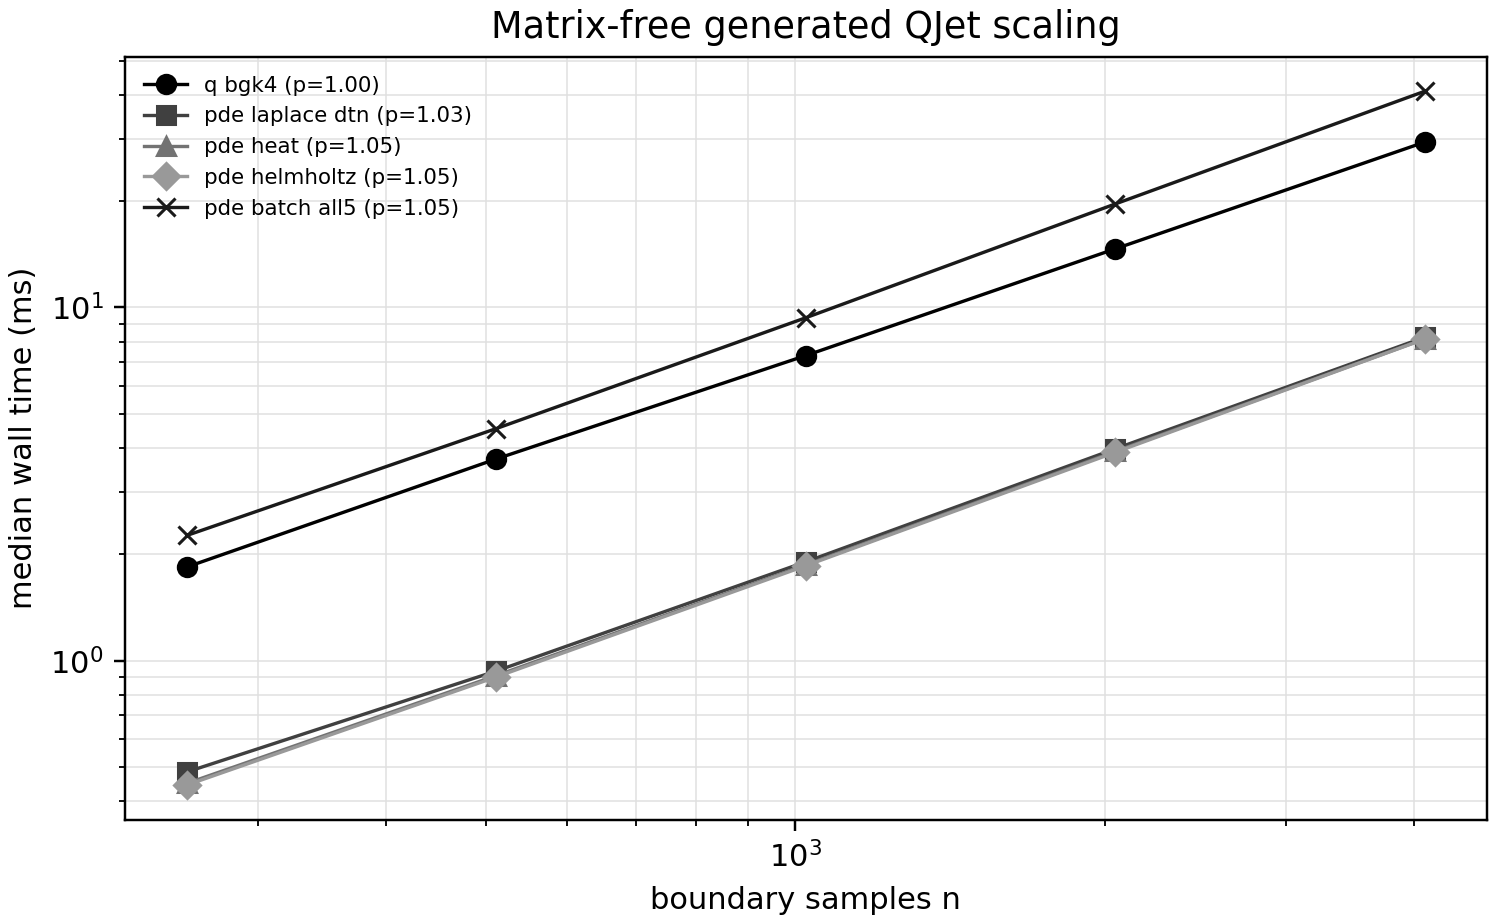
\includegraphics[width=0.82\linewidth]{figures/matrix_free_scaling.png}
\caption{Measured matrix-free scaling.  No dense Q matrix is stored in this sweep.}
\end{figure}
\section{Polygon Smooth-Arc Continuity Ledger}
Polygonal inputs are represented as smooth local arcs for the compute step and then corrected by replacing the arc contribution with exact polygon edge stubs.  The machine-precision entries are therefore a local continuity repayment result, not a free analytic conformal map through corners.
\par\noindent\resizebox{\linewidth}{!}{%
\begin{tabular}{lrrrr}
\toprule
shape & target & panels & smooth arc err & corrected err \\
\midrule
l\_notch & corner & 96 & 0.028 & 1.802e-16 \\
l\_notch & edge & 192 & 0.083 & 2.169e-15 \\
square & corner & 48 & 0.039 & 0 \\
square & edge & 48 & 0.100 & 3.046e-15 \\
star & corner & 192 & 0.038 & 1.322e-15 \\
star & edge & 192 & 0.035 & 8.068e-16 \\
stealth\_double\_concave & corner & 192 & 0.073 & 1.259e-14 \\
stealth\_double\_concave & edge & 192 & 1.436 & 2.647e-13 \\
\bottomrule
\end{tabular}
}\par
\begin{figure}[H]\centering
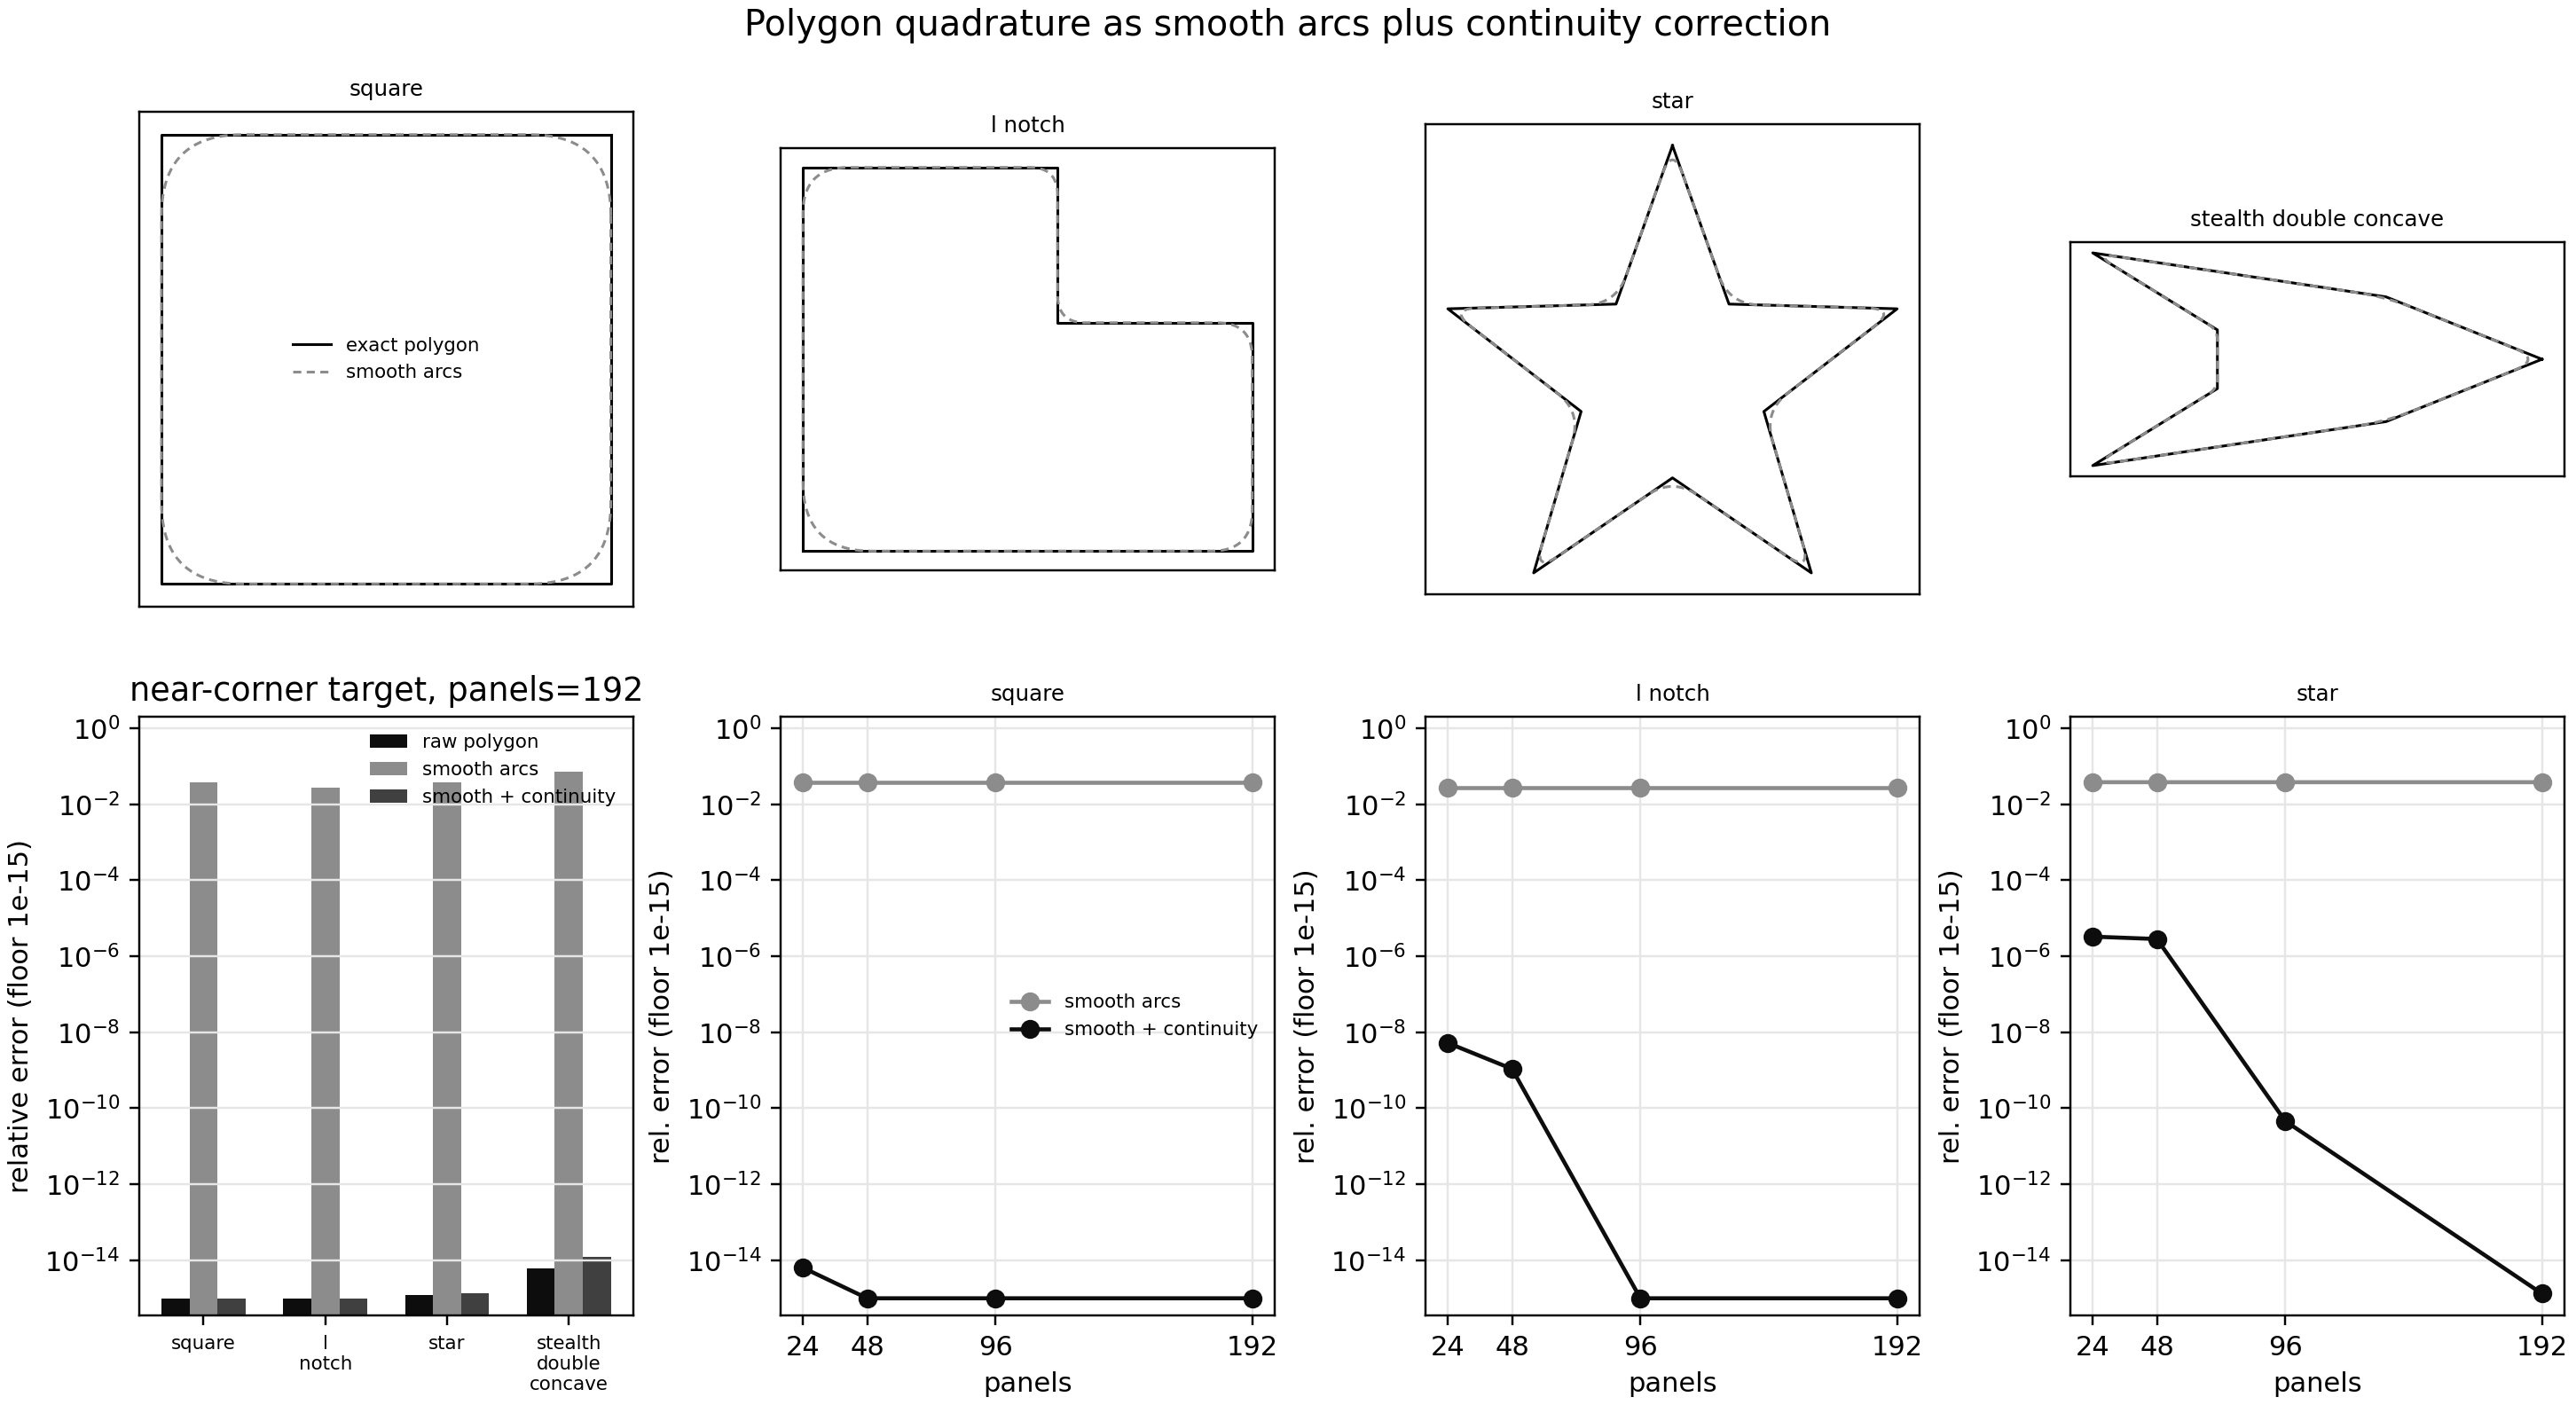
\includegraphics[width=0.90\linewidth]{figures/polygon_continuity.png}
\caption{Polygon continuity correction as a corner repayment layer.}
\end{figure}
\section{Head-to-Head Against QBX and Other Methods}
The structural method benchmark still shows multipole/zeta Q as the preferred robust quadrature path in this corpus.  QBX is strong where its expansion geometry is valid, but it has explicit source-free disk failures at cusp tips.
\par\noindent\resizebox{\linewidth}{!}{%
\begin{tabular}{lrrrrr}
\toprule
method & median err & median ms & work & failures & improvement \\
\midrule
adaptive\_panel & 2.961e-04 & 1.098 & 926.000 & 0 & 36.940 \\
gulati\_q\_bridge & 4.534e-04 & 0.890 & 513.000 & 0 & 12.823 \\
multipole\_zeta\_q & 1.435e-06 & 18.445 & 6.662e+04 & 0 & 5073.817 \\
qbx\_refined & 9.068e-05 & 27.641 & 2.458e+05 & 3 & 159.589 \\
singularity\_subtraction & 4.998e-04 & 0.916 & 533.000 & 0 & 11.182 \\
trapezoid & 0.011 & 0.628 & 512.000 & 0 & 1.000 \\
\bottomrule
\end{tabular}
}\par

\begin{tabular}{lr}
\toprule
quantity & value \\
\midrule
QBX failure rows & 8 \\
QBX median ms & 25.886 \\
QBX median work & 2.458e+05 \\
multipole/zeta Q median ms & 21.912 \\
multipole/zeta Q single-target work & 6.661e+04 \\
tip multipole/zeta improvement & 4.495 \\
near-tip multipole/zeta improvement & 4031.897 \\
\bottomrule
\end{tabular}
\begin{figure}[H]\centering
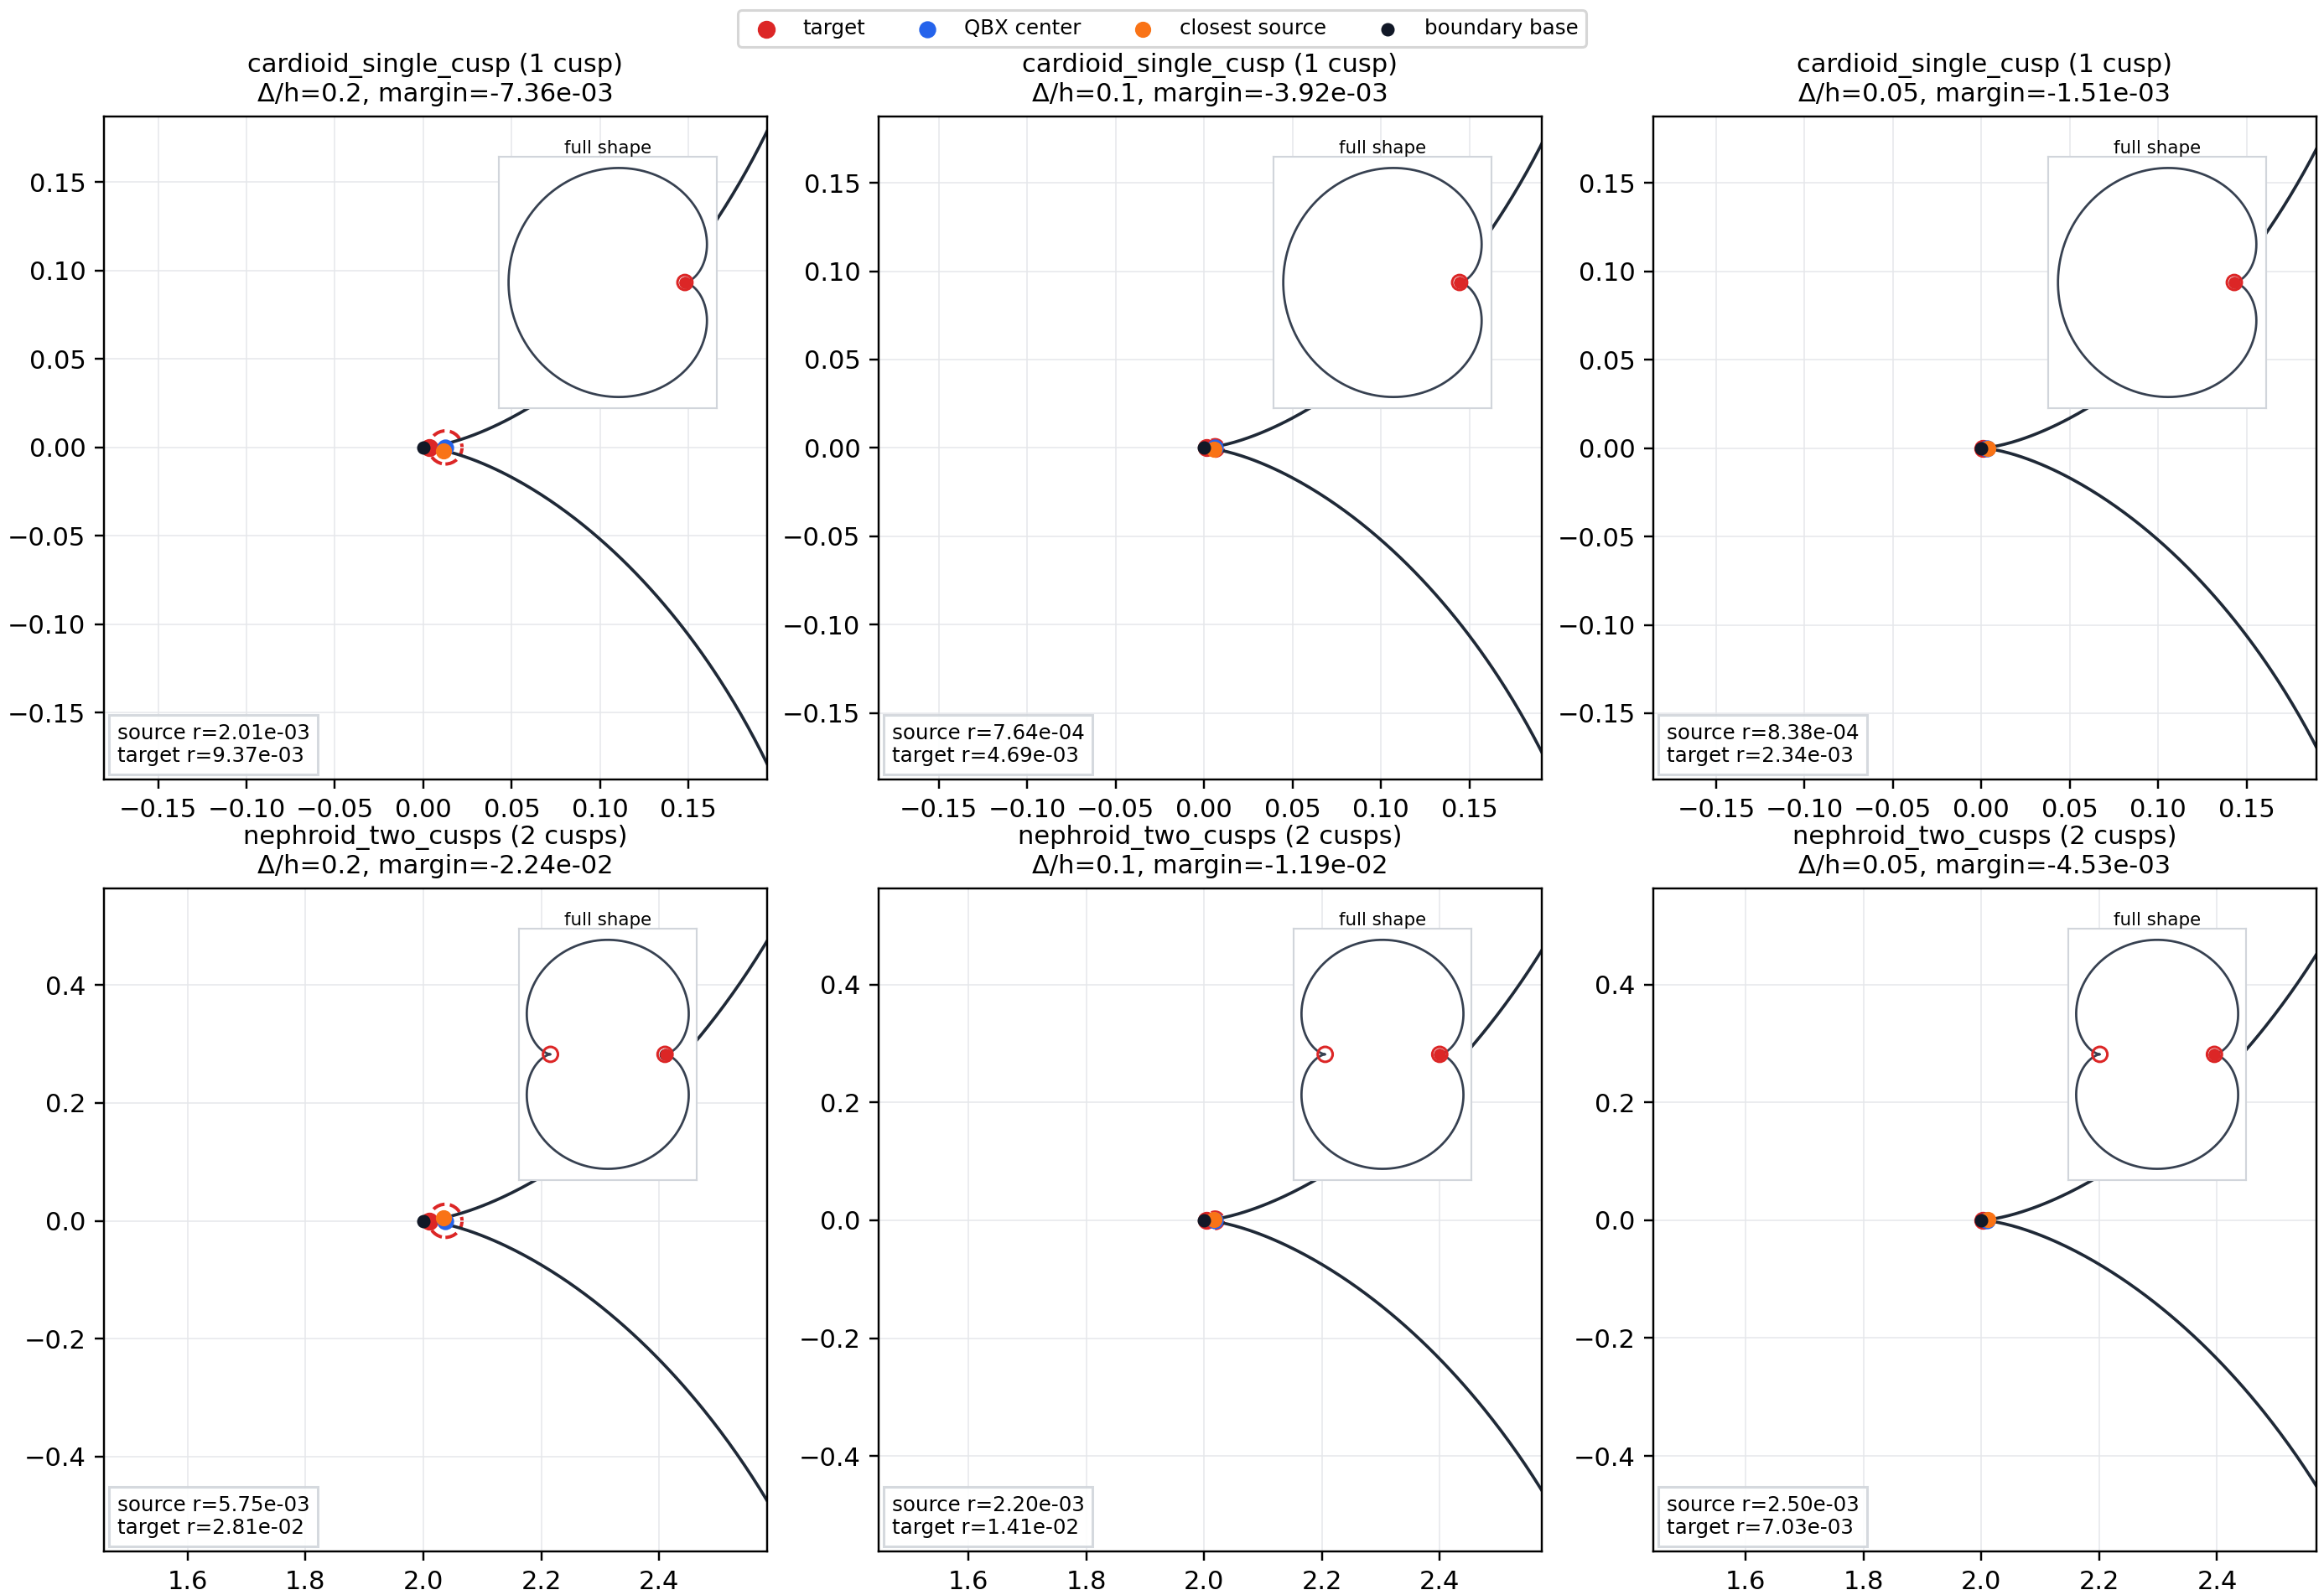
\includegraphics[width=0.85\linewidth]{figures/qbx_failures.png}
\caption{QBX expansion-disk failures at one-cusp and two-cusp geometries.}
\end{figure}
\section{Where FEM Still Beats Q}
The Helmholtz data should be positioned carefully.  Against manufactured exact boundary data, Q wins almost everywhere.  Near resonant volumetric Helmholtz comparisons, FEM can still win in a nontrivial subset.  That is not contradictory: the Q path is a boundary spectral model, while the FEM Schur comparison includes a volumetric discretization and resonance conditioning.
\begin{tabular}{ll}
\toprule
suite & result \\
\midrule
disk modal exact & 14 Q wins / 1 FEM wins \\
manufactured exact & 39 Q wins / 1 FEM wins \\
hard resonance sweep & 256 Q wins / 32 FEM wins \\
median Q manufactured err & 2.077e-08 \\
median FEM manufactured err & 0.175 \\
max Q/FEM error ratio in FEM wins & 35.976 \\
\bottomrule
\end{tabular}
\section{GWW Isospectral Pair: Exact Q Ritz Values}
The continuum Dirichlet spectra of the GWW pair are classically equal.  The experiment below is deliberately narrower: at the discretized chord-operator level, the projected Q spectra separate robustly under refinement.
\begin{verbatim}
left raw clockwise:  [(-3,-3),(-3,-1),(1,3),(1,1),(3,1),(1,-1),(-1,-1),(-1,-3)]
right raw clockwise: [(-3,1),(1,1),(1,3),(3,1),(1,-1),(-1,-1),(-1,-3),(-3,-1)]
orientation: raw lists are reversed to counterclockwise, then centered and scaled to unit area.
nodes: equal arclength s_k=((k+alpha) mod n)L/n with alpha=1/2 midpoint sampling.
corners: exact polygon vertices are kept; midpoint nodes avoid duplicate corner nodes.
normalization: (Lambda_Q,n f)_i=(L/(pi n)) sum_{j!=i}(f_i-f_j)/|x_i-x_j|^2.
\end{verbatim}
\begingroup\small
\begin{tabular}{rp{0.12\linewidth}p{0.34\linewidth}p{0.34\linewidth}}
\toprule
n & relative split & left Ritz 1-6 & right Ritz 1-6 \\
\midrule
256 & 0.074181 & 12.347247, 9.541285, 8.600518, 7.882560, 7.091863, 6.568458 & 11.416318, 10.828102, 8.349505, 7.971254, 7.088097, 6.470439 \\
512 & 0.073772 & 12.420724, 9.607645, 8.656230, 7.927568, 7.147072, 6.605741 & 11.474881, 10.885889, 8.416307, 8.031632, 7.128456, 6.505546 \\
1024 & 0.073513 & 12.456167, 9.640813, 8.685202, 7.949908, 7.174860, 6.624605 & 11.505483, 10.914669, 8.450067, 8.061835, 7.148996, 6.522986 \\
2048 & 0.073364 & 12.472750, 9.657153, 8.700025, 7.960903, 7.188767, 6.634096 & 11.521617, 10.929578, 8.467022, 8.076684, 7.159376, 6.531674 \\
4096 & 0.073287 & 12.481230, 9.665417, 8.707539, 7.966427, 7.195745, 6.638862 & 11.529682, 10.936921, 8.475543, 8.084203, 7.164597, 6.536008 \\
\bottomrule
\end{tabular}
\endgroup
\begin{figure}[H]\centering
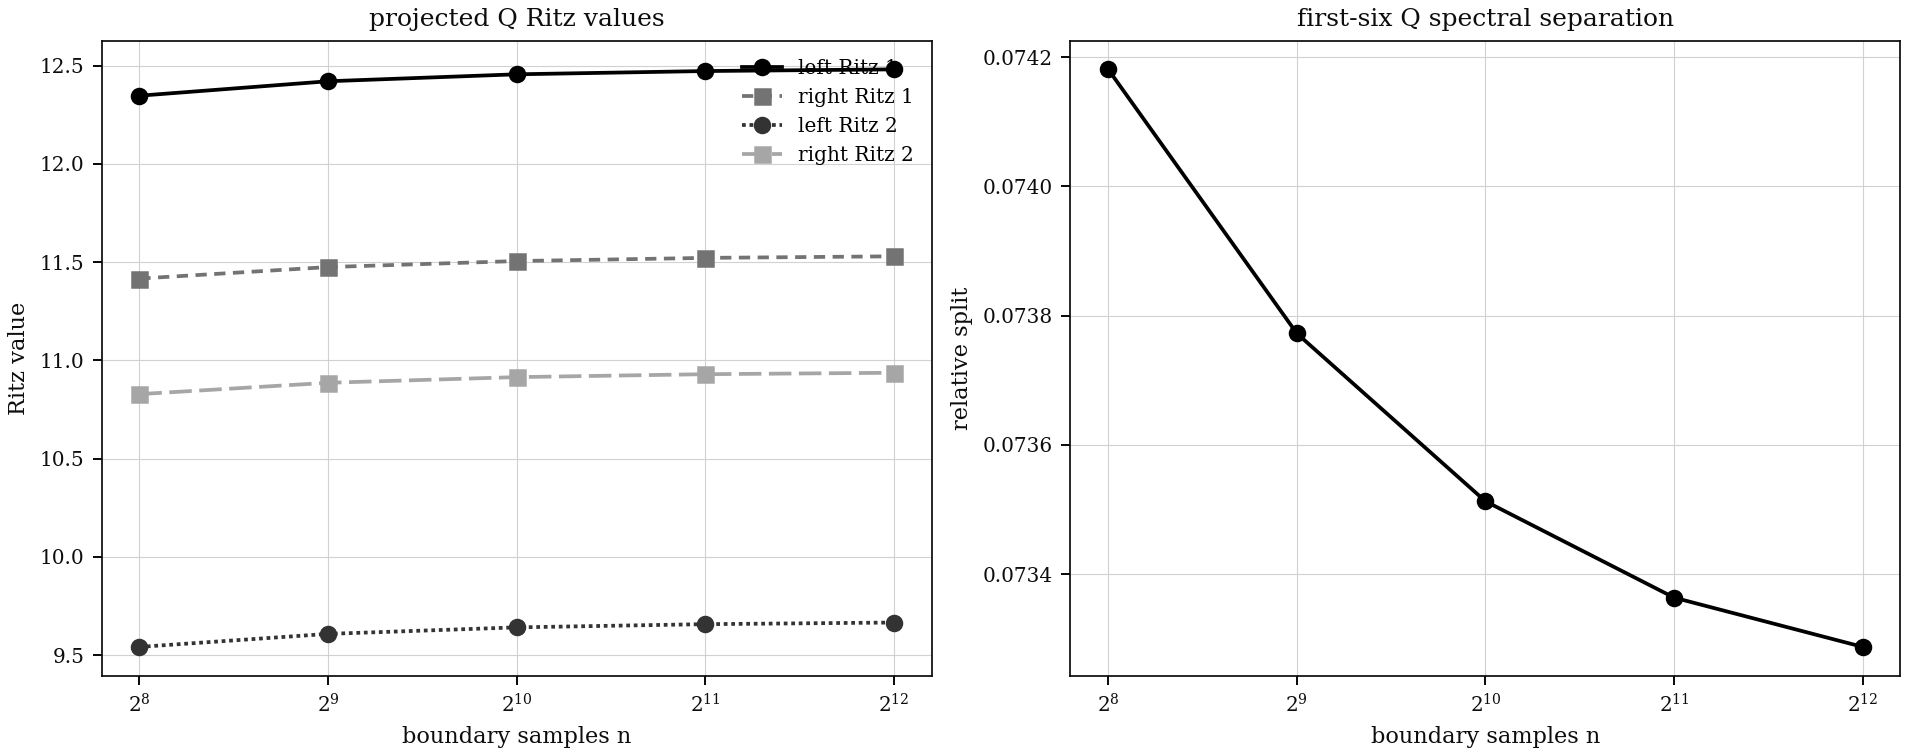
\includegraphics[width=0.92\linewidth]{figures/gww.png}
\caption{GWW projected Q-spectral separation and refinement.}
\end{figure}
\section{Q Spectrum and Error Type}
The Q spectrum is reported as a diagnostic, not just a convergence plot.  High condition proxies and split low modes correlate with corner/cusp channels where multipole/zeta or Mellin corrections are needed.
\begingroup\small
\par\noindent\resizebox{\linewidth}{!}{%
\begin{tabular}{llrrrrr}
\toprule
shape & family & lambda1 & lambda2 & lambda4 & largest & cond proxy \\
\midrule
circle & smooth normal form & 127.500 & 127.500 & 254.000 & 8191.727 & 64.249 \\
golden\_ellipse & smooth conic & 167.230 & 167.671 & 331.696 & 1.457e+04 & 87.148 \\
rounded\_square & smooth high-curvature & 227.087 & 327.022 & 421.130 & 3.177e+04 & 139.886 \\
flower\_nonconvex & smooth nonconvex & 146.592 & 146.891 & 288.939 & 2.233e+04 & 152.354 \\
cardioid\_one\_cusp & cusp & 301.418 & 355.049 & 621.767 & 6.390e+07 & 2.120e+05 \\
nephroid\_two\_cusps & multi-cusp & 305.395 & 415.620 & 648.333 & 1.263e+07 & 4.135e+04 \\
astroid\_four\_cusps & multi-cusp & 440.715 & 550.356 & 779.173 & 3.164e+06 & 7179.138 \\
joukowski\_airfoil & Joukowski cusp & 539.731 & 680.914 & 919.042 & 2.121e+07 & 3.929e+04 \\
square\_polygon & polygonal corners & 159.317 & 159.317 & 317.361 & 1.264e+04 & 79.346 \\
star\_polygon & re-entrant polygon & 108.748 & 108.750 & 216.293 & 1.555e+04 & 143.029 \\
double\_concave\_stealth & concave polygon & 260.672 & 260.693 & 518.359 & 6.704e+04 & 257.170 \\
rational\_asymptote\_chart & open rational chart & 1248.684 & 1248.707 & 2487.623 & 8.068e+04 & 64.610 \\
\bottomrule
\end{tabular}
}\par
\endgroup
\begin{figure}[H]\centering
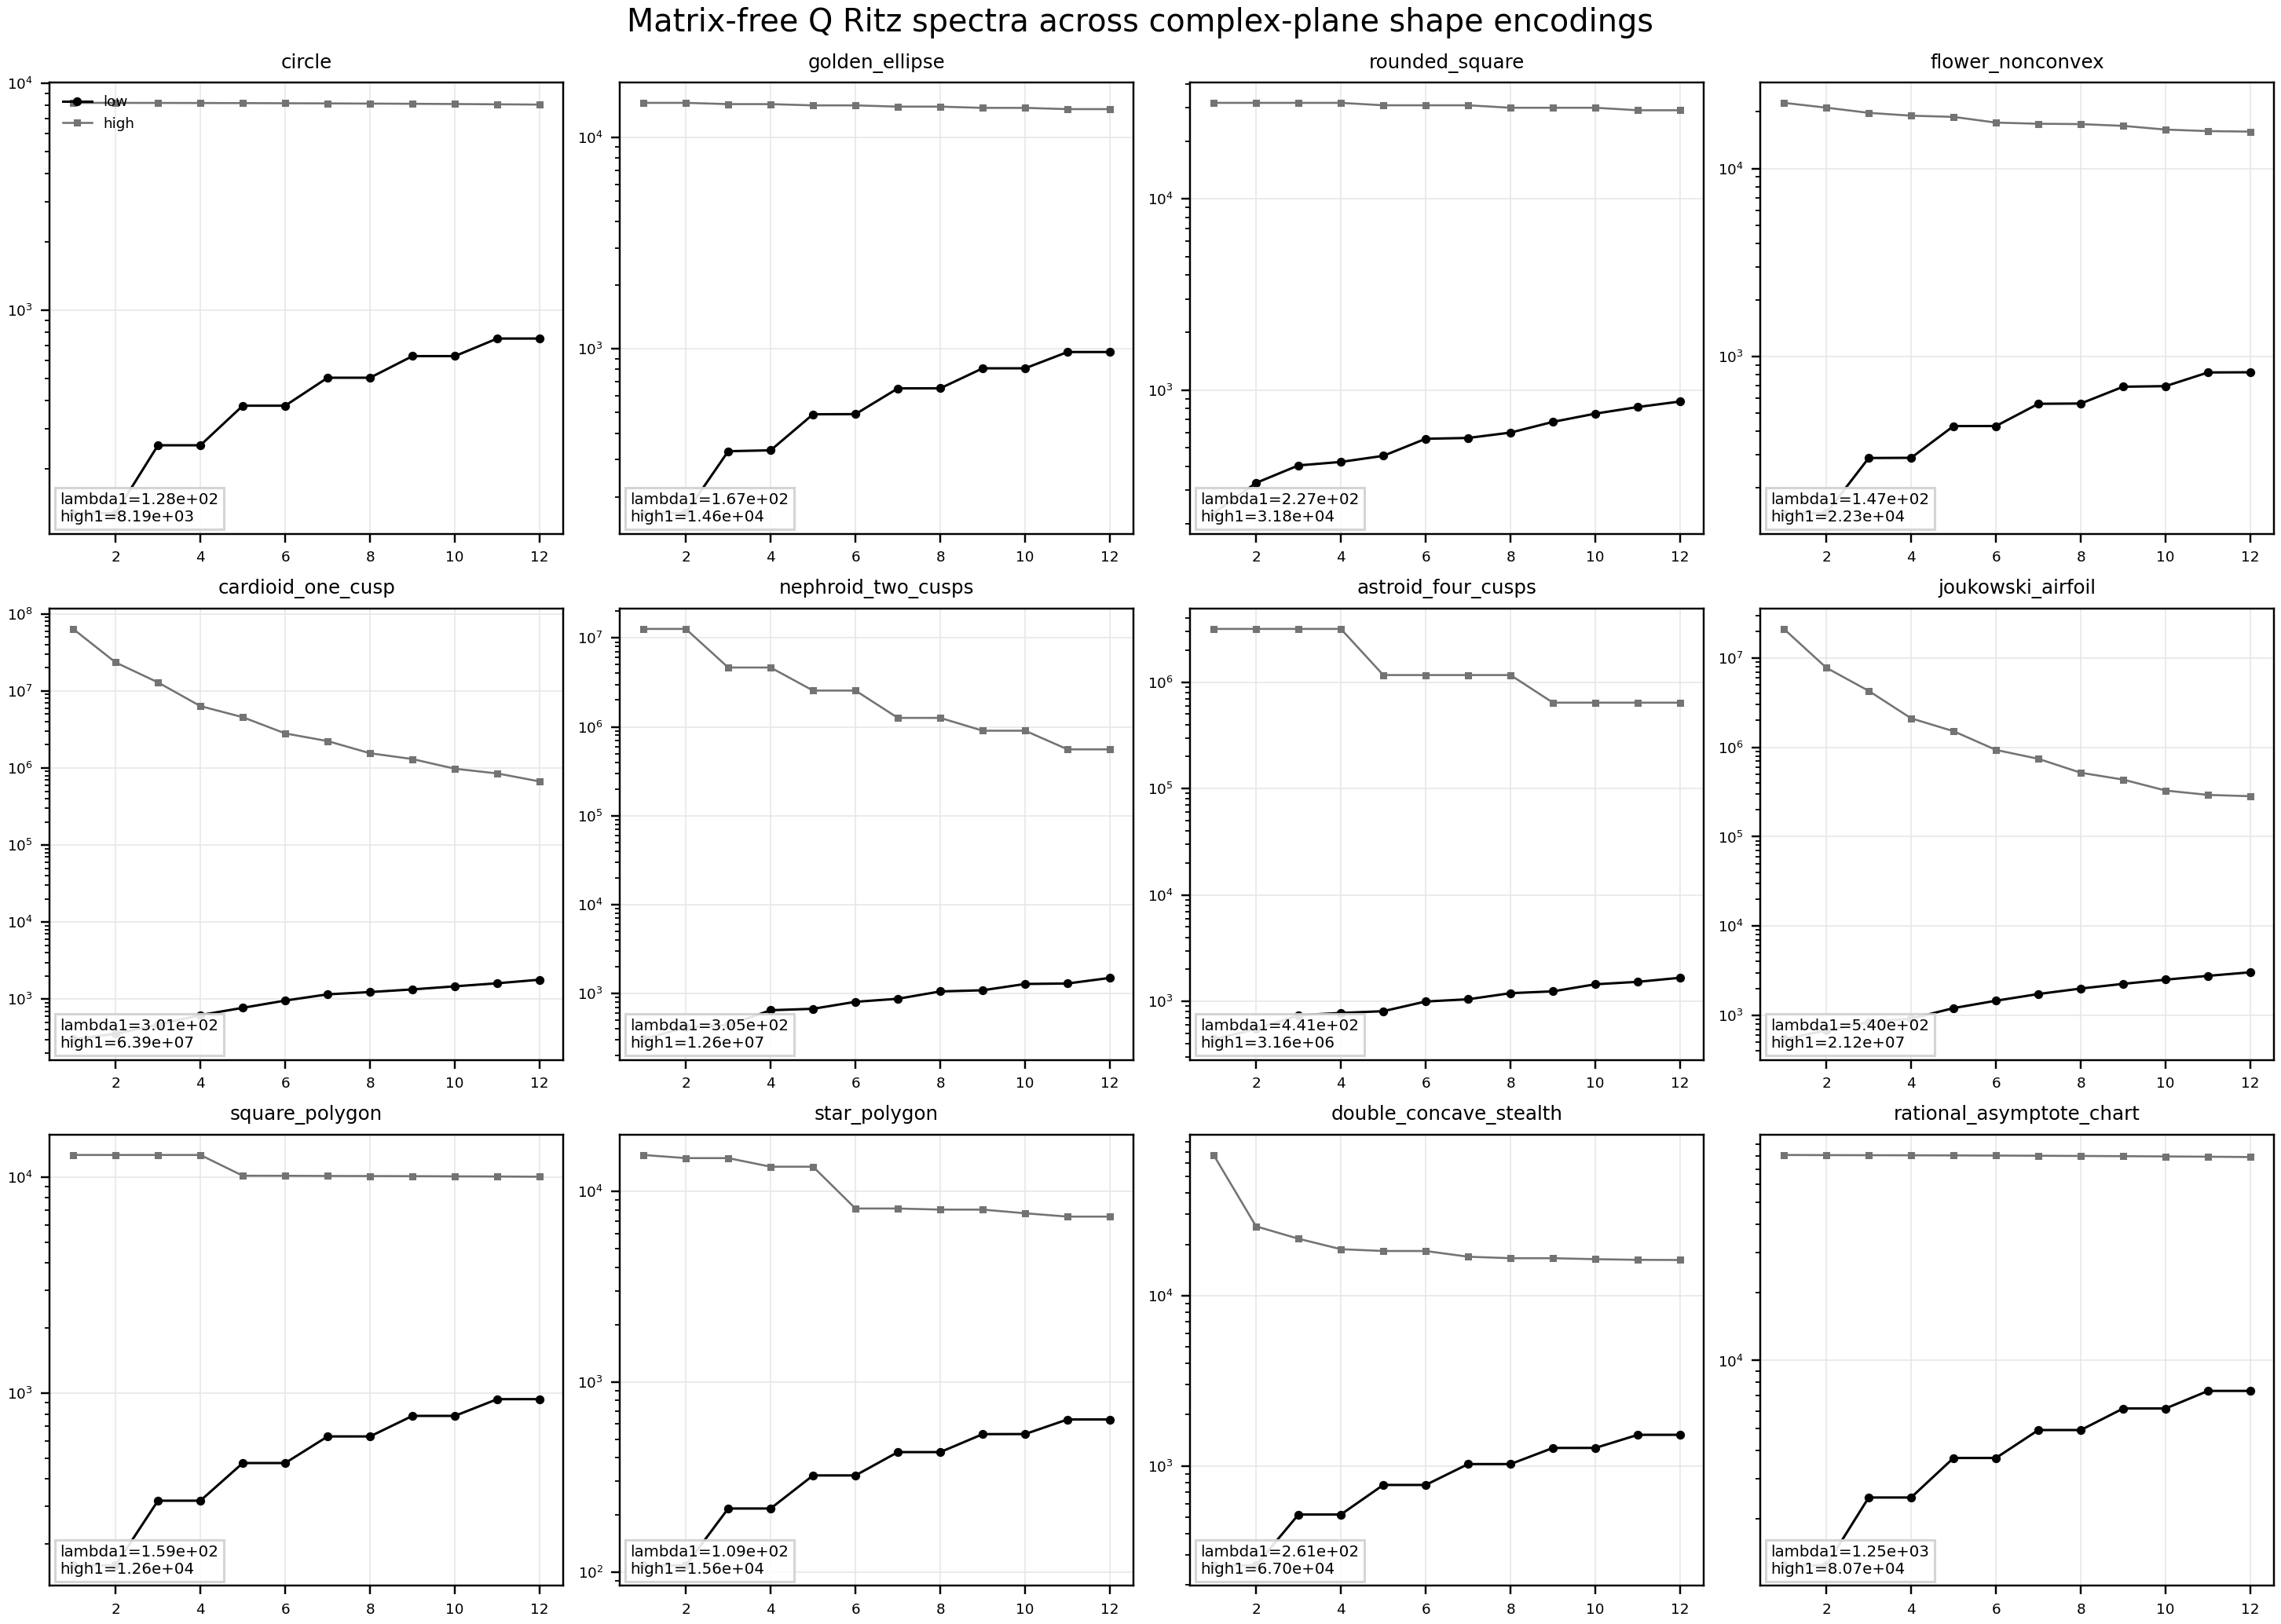
\includegraphics[width=0.95\linewidth]{figures/spectrum_gallery.png}
\caption{Exact computed Q Ritz spectrum gallery.}
\end{figure}
\section{BGK Endpoint Bookkeeping}
The endpoint ledger identifies the same constant in Monte Carlo barrier crossing, DtN spectral endpoint sums, and the chord-to-arc correction channel.  This is the conceptual reason the BGK layer belongs in the Q pipeline.
\begin{figure}[H]\centering
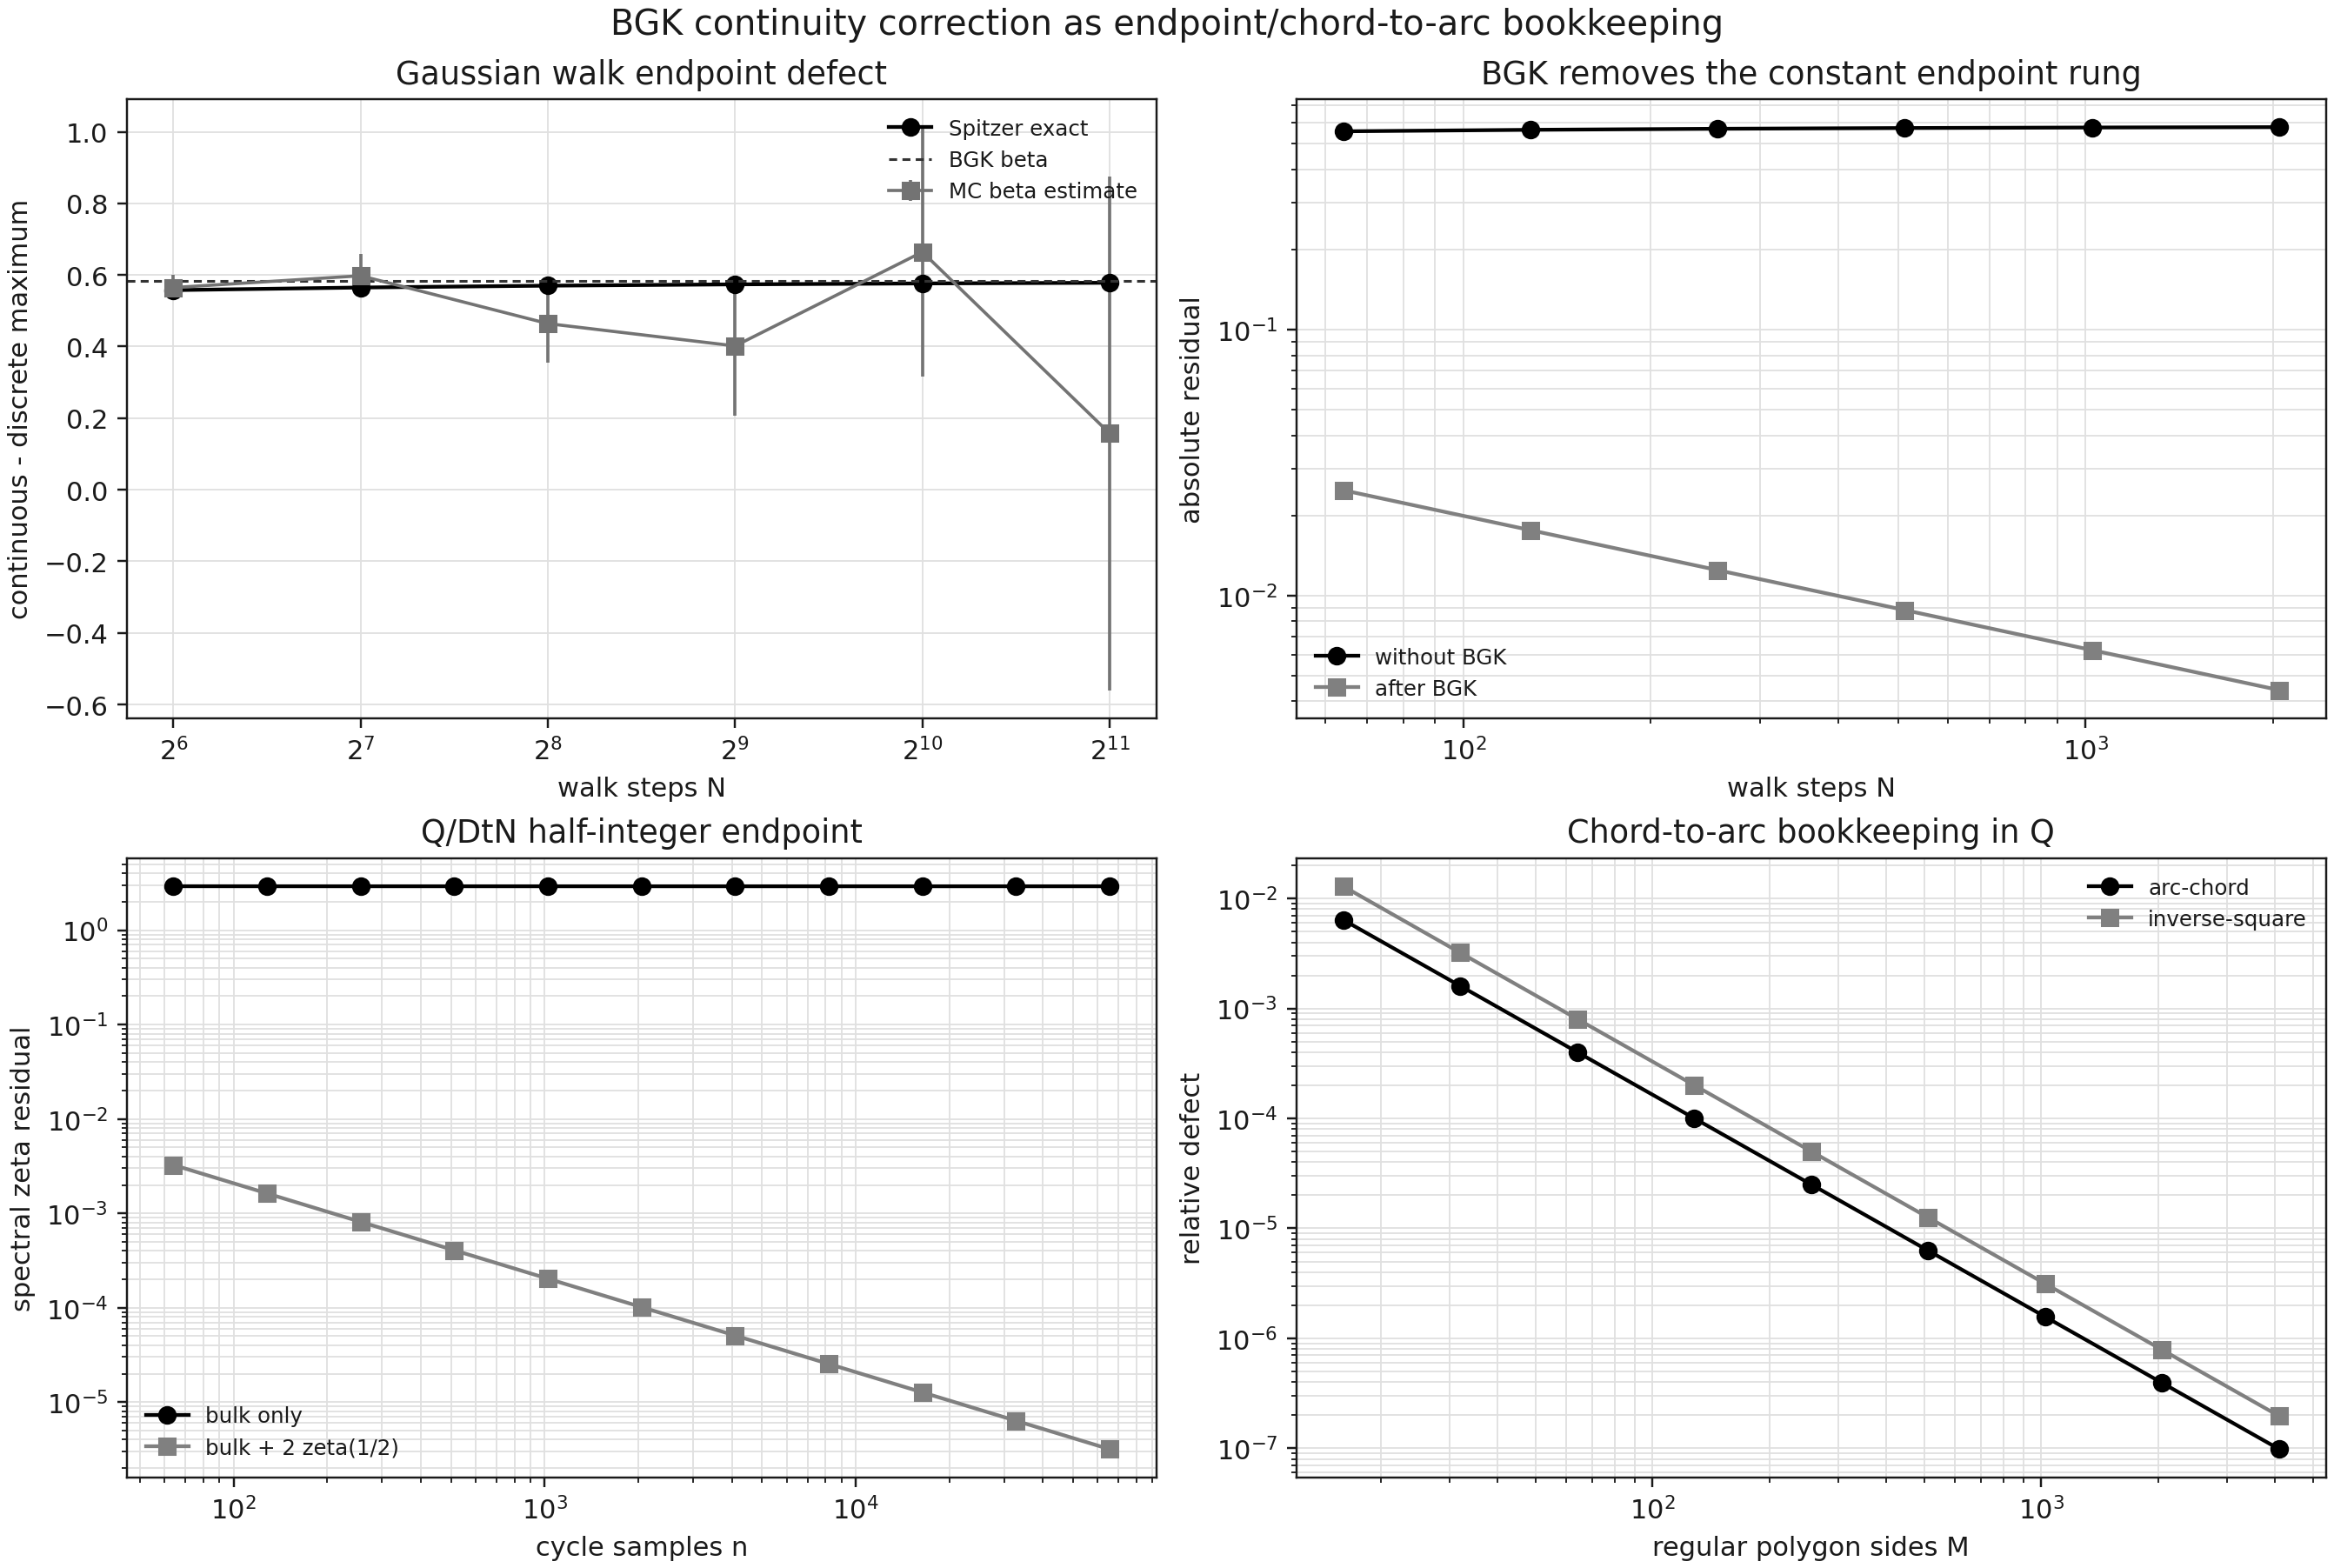
\includegraphics[width=0.90\linewidth]{figures/bgk_bookkeeping.png}
\caption{BGK endpoint bookkeeping: Spitzer, zeta, and Q/DtN endpoints.}
\end{figure}
\section{Reproducibility}
\begin{verbatim}
python3 examples/pullback/exterior_kernel_split_qrule_benchmark.py
python3 examples/pullback/exterior_q_bgk_correction_pipeline.py
python3 examples/pullback/funky_shape_q_bgk_pde_suite.py
python3 examples/corners/polygon_smooth_arc_continuity_benchmark.py
python3 examples/isospectral/gww_section11_audit.py
python3 examples/q_spectrum_shape_gallery.py
python3 scripts/build_machine_precision_pipeline_report.py
\end{verbatim}
Generated artifacts live under \texttt{outputs/machine\_precision\_pipeline\_report}.
\end{document}
